%%%%%%%%%%%%%%%%%%%%%%%%%%%%%%%%%%%%%%%%%%%%%%%%%%%%%%%%%%%%%%%%%%%%%%%%%%%%%%%%
% Template for USENIX papers.
%
% History:
%
% - TEMPLATE for Usenix papers, specifically to meet requirements of
%   USENIX '05. originally a template for producing IEEE-format
%   articles using LaTeX. written by Matthew Ward, CS Department,
%   Worcester Polytechnic Institute. adapted by David Beazley for his
%   excellent SWIG paper in Proceedings, Tcl 96. turned into a
%   smartass generic template by De Clarke, with thanks to both the
%   above pioneers. Use at your own risk. Complaints to /dev/null.
%   Make it two column with no page numbering, default is 10 point.
%
% - Munged by Fred Douglis <douglis@research.att.com> 10/97 to
%   separate the .sty file from the LaTeX source template, so that
%   people can more easily include the .sty file into an existing
%   document. Also changed to more closely follow the style guidelines
%   as represented by the Word sample file.
%
% - Note that since 2010, USENIX does not require endnotes. If you
%   want foot of page notes, don't include the endnotes package in the
%   usepackage command, below.
% - This version uses the latex2e styles, not the very ancient 2.09
%   stuff.
%
% - Updated July 2018: Text block size changed from 6.5" to 7"
%
% - Updated Dec 2018 for ATC'19:
%
%   * Revised text to pass HotCRP's auto-formatting check, with
%     hotcrp.settings.submission_form.body_font_size=10pt, and
%     hotcrp.settings.submission_form.line_height=12pt
%
%   * Switched from \endnote-s to \footnote-s to match Usenix's policy.
%
%   * \section* => \begin{abstract} ... \end{abstract}
%
%   * Make template self-contained in terms of bibtex entires, to allow
%     this file to be compiled. (And changing refs style to 'plain'.)
%
%   * Make template self-contained in terms of figures, to
%     allow this file to be compiled. 
%
%   * Added packages for hyperref, embedding fonts, and improving
%     appearance.
%   
%   * Removed outdated text.
%
%%%%%%%%%%%%%%%%%%%%%%%%%%%%%%%%%%%%%%%%%%%%%%%%%%%%%%%%%%%%%%%%%%%%%%%%%%%%%%%%

\documentclass[letterpaper,twocolumn,10pt]{article}
\usepackage{usenix}

% to be able to draw some self-contained figs
\usepackage{tikz}
\usepackage{amsmath}

% inlined bib file
\usepackage{filecontents}


\usepackage{mathptmx} % This is Times font
\usepackage{comment}
%\usepackage{fancyhdr}
\usepackage[font={small}]{caption}
\usepackage[normalem]{ulem}
%\usepackage[hyphens]{url}
\usepackage{amsmath}
\usepackage{amssymb}
\usepackage{graphicx}
\usepackage{pifont}
 \usepackage{algorithm}
\usepackage{xcolor}
\usepackage{rotating}
\usepackage{titling}
% %\usepackage{algorithm2e}
\usepackage[utf8]{inputenc}
%\usepackage{fourier} 
\usepackage{array}
\usepackage{makecell}
\renewcommand\theadalign{bc}
\renewcommand\theadfont{\bfseries}
\renewcommand\theadgape{\Gape[4pt]}
\renewcommand\cellgape{\Gape[4pt]}
\newcommand{\bikash}[1]{\COMMENT{\textcolor{blue}{\sf Bikash: #1}}}
\usepackage{wrapfig}
\usepackage[noend]{algpseudocode}
\usepackage{float}
\usepackage{color}
% \usepackage[space]{cite}
\usepackage{tabularx}
\usepackage{subcaption} 
% % \captionsetup{compatibility=false}
% % \usepackage{tikz}
% % \usepackage{url}
% % \usepackage{soul}
\usepackage{enumitem}
% \usepackage{natbib}
\usepackage{multirow}
\frenchspacing
\usepackage{microtype}

\algdef{SE}[FOR]{NoDoFor}{EndFor}[1]{\algorithmicfor\ #1}{\algorithmicend\ \algorithmicfor}%
\algdef{SE}[IF]{NoThenIf}{EndIf}[1]{\algorithmicif\ #1}{\algorithmicend\ \algorithmicif}%
\newcommand*\circled[1]{\tikz[baseline=(char.base)]{
  \node[shape=circle,draw,fill=black,text=white,font=\bf,inner sep=0.5pt] (char)
  {\scriptsize#1};
}}

\newcommand*\circledwhite[1]{\tikz[baseline=(char.base)]{
  \node[shape=circle,draw,fill=white,text=black,font=\bf,inner sep=0.5pt] (char)
  {\scriptsize#1};
}}

\newcommand{\putsec}[2]{\vspace{-0.0in}\section{#2}\label{sec:#1}\vspace{-0.0in}}
\newcommand{\putssec}[2]{\vspace{-0.0in}\subsection{#2}\label{ssec:#1}\vspace{-0.0in}}
\newcommand{\putsssec}[2]{\vspace{-0.0in}\subsubsection{#2}\label{sssec:#1}\vspace{-0.0in}}
%\newcommand{\putsssecX}[1]{\vspace{0.0in}\subsubsection*{#1}\vspace{0.0in}}
\newcommand{\putsssecX}[1]{\vspace{0.0in}\noindent\textbf{#1:}}

\newcommand{\figref}[1]{Figure~\ref{fig:#1}}
\newcommand{\eqnref}[1]{Equation~\ref{eq:#1}}
\newcommand{\tabref}[1]{Table~\ref{tab:#1}}
\newcommand{\secref}[1]{Section~\ref{sec:#1}}
\newcommand{\ssecref}[1]{Section~\ref{ssec:#1}}
\newcommand{\sssecref}[1]{Section~\ref{sssec:#1}}

\newcommand{\COMMENT}[1]{#1}
\newcommand{\prash}[1]{\COMMENT{\textcolor{blue}{\sf Prash: #1}}}
\newcommand{\ashu}[1]{\COMMENT{\textcolor{green}{\sf Ashutosh: #1}}}
\newcommand{\nachi}[1]{\COMMENT{\textcolor{green}{\sf Nachi: #1}}}
\newcommand{\jash}[1]{\COMMENT{\textcolor{green}{\sf Jashwant: #1}}}
\newcommand{\das}[1]{\COMMENT{\textcolor{red}{\sf Dr.Das: #1}}}
\newcommand{\mahmut}[1]{\COMMENT{\textcolor{red}{\sf Dr.Kandemir: #1}}}
\newcommand\pras[1]{\textcolor{Green}{{\bf Prasanna:} #1}}
\newcommand\bsharma[1]{\textcolor{red}{{\bf Bikash:} #1}}
\newcommand{\todo}[1]{\COMMENT{{\color{red}\sf\bfseries #1}}}
\makeatletter
\renewcommand{\p@subsection}{}
\renewcommand{\p@subsubsection}{}
\makeatother

\renewcommand{\footnoterule}{
  \kern -3pt
  \hrule width 0.49\textwidth height 1pt
  \kern 2pt
}

\newcommand{\cmark}{\ding{51}}
\newcommand{\xmark}{\ding{55}}
\newcommand{\ignore}[1]{}

% Uncomment this to remove the inline comments
%\renewcommand{\COMMENT}[1]{}

\usepackage{lipsum}
\setlength{\textfloatsep}{9pt plus 1.0pt minus 3.0pt}
\setlength{\floatsep}{5pt plus 1.0pt minus 2.0pt}
\setlength{\intextsep}{5pt plus 1.0pt minus 2.0pt}
\setlength{\droptitle}{-70pt}
%\posttitle{\par\end{center} \vskip -5.5em}

%-------------------------------------------------------------------------------
\begin{document}
%-------------------------------------------------------------------------------

%don't want date printed
\date{}

% make title bold and 14 pt font (Latex default is non-bold, 16 pt)
\title{\Large \bf Kube-Knots: Dynamic Container Orchestration and Resource Management for GPU-based Datacenters}

%%for single author (just remove % characters)
%\author{
%{\rm Your N.\ Here}\\
%Your Institution
%\and
%{\rm Second Name}\\
%Second Institution
%% copy the following lines to add more authors
%% \and
%% {\rm Name}\\
%%Name Institution
%} % end author

\maketitle

%-------------------------------------------------------------------------------
\begin{abstract}
%-------------------------------------------------------------------------------
Compute heterogeneity in the form of accelerators like GPUs and FPGAs is increasingly gaining prominence in modern datacenters. We observe that datacenter schedulers are agnostic of these emerging accelerators and their resource footprints, and thus, not well equipped to dynamically orchestrate them by providing fine-grained resource guarantees to latency sensitive applications. 
%such user-facing queries as they are agnostic of the GPU usage metrics. 
This also causes several resource fragmentation and interference issues leading to overall resource under-utilization. Furthermore, since these accelerators are not power proportional, proactive management of these resources by the cluster-wide resource orchestrator is essential to keep the operational costs low and ensuring the Quality of Service (QoS).

In this paper, we identify the challenges in developing a GPU-aware datacenter scheduler and explore the potential opportunities that arise by exposing GPU APIs to the datacenter scheduler. Based on our observations from Alibaba's cluster traces and real hardware GPU cluster experiments, we build \textit{Knots}, a GPU-aware resource orchestrator and integrate it with \textit{Kubernetes} container orchestrator. We evaluate three GPU-based scheduling techniques to schedule representative GPU workload mixes through \textit{Kube-Knots} on a ten node GPU cluster. Our proposed PP scheduler  improves both 50$^{th}$ and 90$^{th}$ percentile cluster-wide GPU utilization by up to 80\%. This leads to 33\% cluster-wide power savings on an average for three different workloads compared to Kubernetes's default scheduler. At the same time, this ensures the end-to-end QoS of latency critical GPU bound queries by reducing the QoS violation up to 53\% when compared to resource agnostic scheduler.
\end{abstract}


\section{INTRODUCTION} 
\label{sec:intro}

    Modern data centers are increasingly being provisioned with compute accelerators such as GPUs, FPGAs and ASIC's to catch up with the workload performance demands and reduce the total cost of ownership (TCO) \cite{caulfield2016cloud}. By 2021, traffic within hyperscale datacenters is expected to quadruple with 94\% of workloads moving to cloud-based datacenters according to Cisco's global cloud index~\cite{cisco}. Based on the nature of the application, it can either benefit from high throughput of GPUs or low latency of special purpose hardwares such as FPGAs and TPUs~\cite{jouppi2017datacenter}. A majority of them include data mining, image processing, speech recognition and gaming \cite{1659988, Povey11thekaldi,10.1007/11744023_32}, uses GPUs for high throughput computing. This trend is evident as public cloud operators like Amazon \cite{amazon} and Microsoft \cite{microsoft} have started to offer GPU-based infrastructure services.

\begin{figure}[!tbp]
\centering
  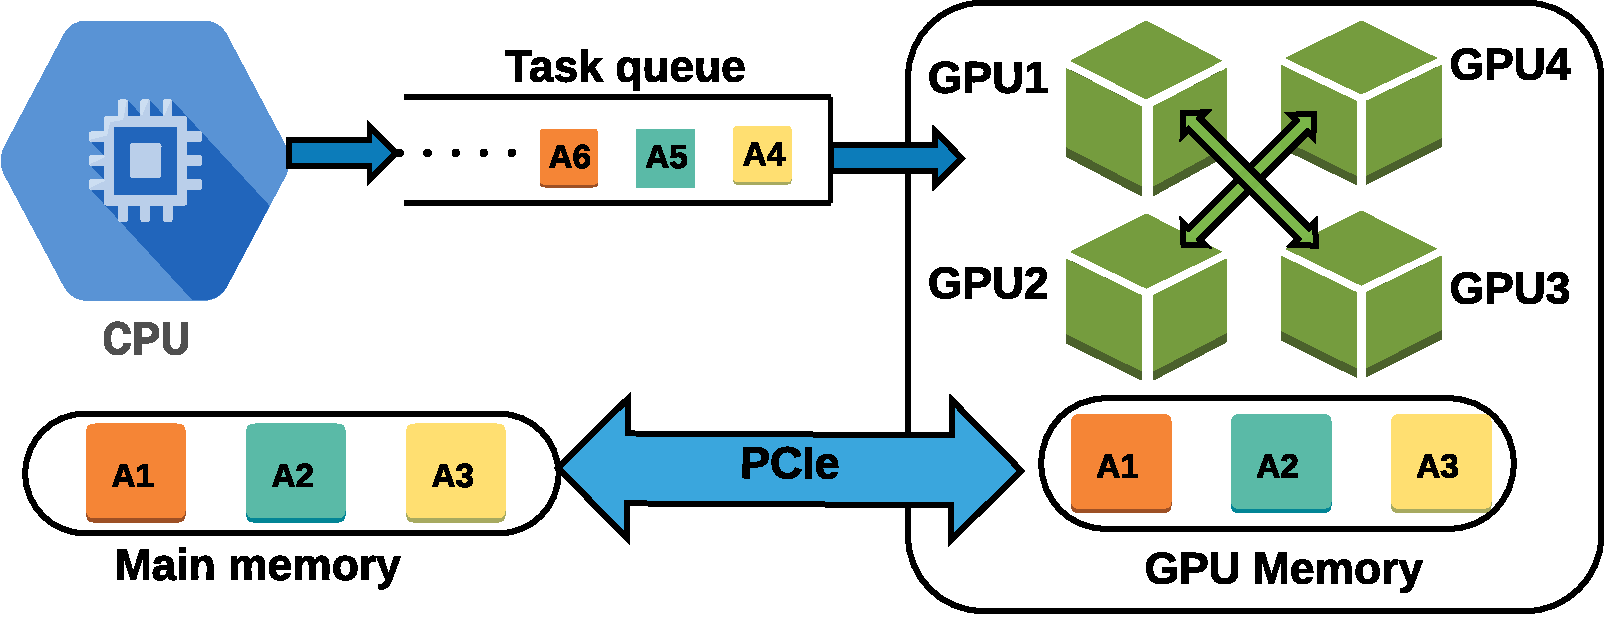
\includegraphics[width=.84\linewidth,height=2.2cm]{figs/cpu-gpu-queue.pdf}
  \vspace{-2mm}
  \caption{Application queue on a single node with multiple GPUs.}
  \vspace{-2mm}
  \label{fig:queue}
\end{figure}

% For example, a wearable health monitoring device aggregates several sensor data through a mobile application. In case of a data anomaly, inference services can be triggered from the mobile device to the cloud, requesting for a deep neural network  (DNN) model that fits the symptom \cite{hauswald2015djinn}. 

A class of emerging workloads in public datacenters, which include user-facing queries (in forms of voice, text and image etc.)  \cite{qualcomm,TjongKimSang:2000:ICS:1117601.1117631,Hearst:2011:NSU:2018396.2018414}, demand sub-millisecond turn around times (such as Siri and Alexa) \cite{siri,alexa} and pose varying compute demands \cite{Hauswald:2015:SOE:2694344.2694347}. These applications, subscribe to datacenter accelerators in the form of queries (e.g. inference requests from a DNN model) \cite{hauswald2015djinn}. These GPU-bound queries impose strict Service Level Agreements (SLAs) that is usually set around 150 to 500ms~\cite{gujarati2017swayam}. In contrast to the regular datacenter batch workloads, these user-facing applications are typically hosted as services that occur and scale in short bursts \cite{Barroso:2009:DCI:1643608,Dean}. Companies like Netflix break down their application compute flow pipeline into several containerized microservices in order to ease scalability and maintenance of the workflow  ~\cite{netflix}. Many of these containerized workloads and microservices subscribe to compute-intensive frameworks such as Tensorflow~\cite{tensor}, Caffe~\cite{jia2014caffe}, Theano~\cite{Theano}, etc. taking advantage of GPU's high performance API primitives~\cite{ChetlurWVCTCS14}. Note that, these microservices are interconnected with each stage having strict deadlines depends on the application scheduler to meet the tight performance bounds. With the expected increase in such workloads~\cite{cisco}, the GPU resource scheduling problem is expected to exacerbate. Hence, GPUs/accelerators are on the critical path to ensure the performance, and meet end-to-end latency demands of such queries.
% MATLAB \cite{Dean,Weideman:2000:MDM:365723.365727},

Also, we identify that the GPU-agnostic orchestration and scheduling would violate the strict QoS deadline of these queries. As a result, an efficient management strategy of such compute accelerators across the datacenter becomes crucial. 
%For example, Google Brain project \cite{brain}, which is a DNN based containerized service, is used across teams in Google to reduce the need to maintain different implementations of the same service. This trend is also increasingly common in companies like 
On the other hand, these services if not batched together would also underutilize the GPU~\cite{hauswald2015djinn}. The primary design goal of any efficient cluster manager is to achieve high resource utilization with low job turnaround times. Traditional datacenter operators leverage techniques such as hardware virtualization \cite{Gupta:2011:PCS:2002181.2002184} to improve the overall cluster utilization. To further improve the energy efficiency, the cluster resource orchestrators also employ techniques like workload consolidation or dynamic load balancing through VM migration. However, none of these traditional CPU-based cluster management techniques can be extended to GPU-based datacenters since commodity GPUs can neither be virtualized nor be consolidated because the jobs scheduled to GPUs are not preemptible.\footnote{GPU virtualization in Nvidia Grid is only for graphics pipeline \cite{grid}.}

State-of-the-art resource orchestrators such as Kubernetes \cite{kubernetes} and Mesos \cite{mesos} perform uniform scheduling, which statically assigns the GPU resources to the applications. The scheduled pods access the GPUs via PCIe pass-through, which gives the application complete access to the GPU as seen in Figure~\ref{fig:queue}. Specifically, Kubernetes has support for dynamic orchestration with features such as node affinity, pod\footnote{We use the terms (Google's) pod and container interchangeably.} affinity, and pod preemption for CPUs. However, these features cannot be extended to GPUs as they lack support for pod preemption. In addition, \textit{Kubernetes} lacks the ability to query real-time GPU metrics such as memory, Streaming Multiprocessor(SM is a GPU-core) utilization, PCIe bandwidth, etc. Containers often overstate their GPU resource requirements such as memory, and this leads to severe resource underutilization and QoS violations due to queuing delays~\cite{kang2017convgpu}. To summarize, we list several challenges in managing GPU based datacenters below, %Hence we need to build an orchestration layer which can log the critical metrics and use them with state of the art Kubernetes features to develop a utilization aware and. \jash{strongly mention util problem and emphasize your takeaways} %Since the resource management layer has no control over the GPU utilization or management, the resource fairness is entirely dependent on the application which is currently running on GPU. Hence techniques such as preemption to enforce fairness cannot be applicable in this case.%



% The default scheduling options in kubernetes or Mesos are tuned towards optimizing CPU cluster metrics such as throughput, and overall resource utilization. These schedulers are also agnostic to the heterogeneity available in these architectures, and therefore, lead to suboptimal scheduling.
% However these resource orchestrators like Kubernetes also have provision to plug-in custom scheduling policies based on the specific demands of the datacenter. We propose a need for GPU focused datacenter cluster orchestrator. To meet this need, we discuss the potential challenges in designing a GPU context aware scheduler by exposing the device API's to the kubernetes.


\begin{itemize}[wide, nosep, labelindent = 0pt, topsep = 0.3ex]
\item \textbf{Non-preemptive processing elements -} The containers scheduled to GPUs cannot be preempted, or context switched, or prioritized and are scheduled based on First Come First Serve (FCFS) order~\cite{amert2017gpu} as seen in Figure~\ref{fig:queue}. Therefore, GPU-bound latency sensitive queries when queued behind a batch job will incur severe queuing delays.

\item \textbf{GPU utilization aware scheduler -} Today's datacenter resource orchestrators treat GPU's as a black box and are agnostic of GPU utilization metrics. Meeting the QoS of a latency sensitive query is difficult without knowing the system state, especially when it is shared.

\item \textbf{Unaccountable container performance metrics -} \\Container-level accountability for resource consumption is not enabled in GPUs. This lets the node-level application frameworks like Tensorflow to conservatively over-commit the GPU resources~\cite{tensorflowgpu} resulting in poor energy efficiency %due to resource underutilization.
\item \textbf{Performance per watt proportionality -} GPUs have linear performance per watt scaling, which implies that the maximum energy efficiency can be achieved only when GPUs are 100\% utilized, unlike CPUs \cite{wong2016peak}. It is crucial for a scheduler to fully pack and utilize the GPUs without affecting the individual application performance.
\end{itemize}

\begin{figure}[!tbp]
\centering
  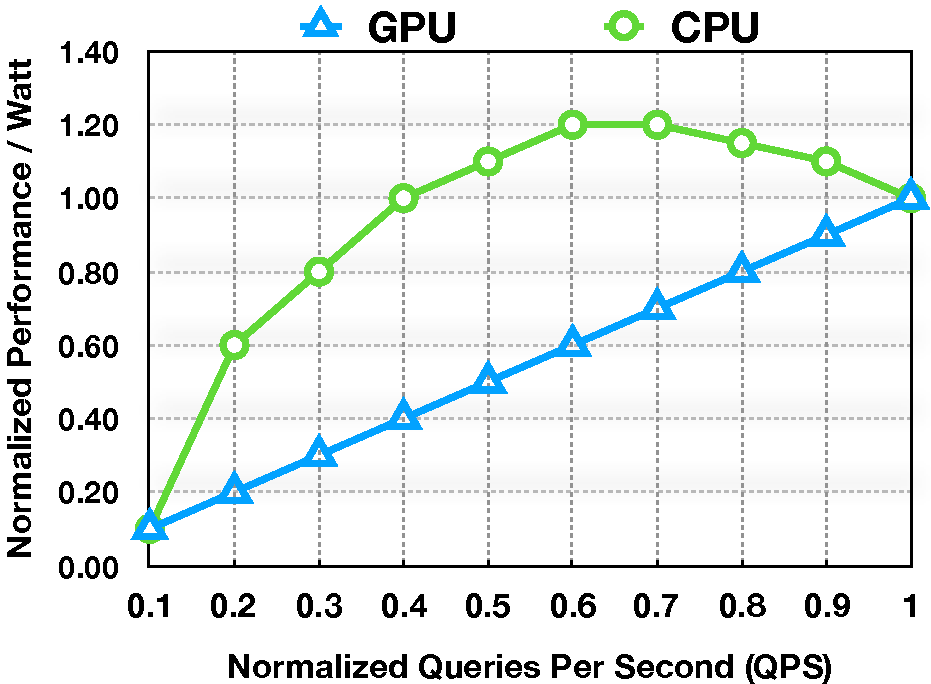
\includegraphics[width=.85\linewidth]{results/energy.pdf}
  \vspace{-2mm}
  \caption{Performance per Watt trend of CPU and GPU serving Memcached queries.}
  \vspace{-2mm}
  \label{fig:efficiency}
\end{figure}

% The challenges listed above pitches a strong case for reducing resource fragmentation through workload consolidation. In case of co-located GPU applications, prediction of the end-to-end latency and QoS of a query becomes difficult. %The schedulers today are agnostic of accelerator device metrics and without specific orchestration or scheduling policy in place, schedulers treat the accelerators as black boxes. They schedule the queries based on FCFS without any bounded performance guarantees. Such resource-agnostic, conservative scheduling policies lead to poor utilizations and are also energy inefficient. 
% \begin{figure*}
% \hspace{-10mm}
% \begin{subfigure}[t!]{.3\textwidth}
%   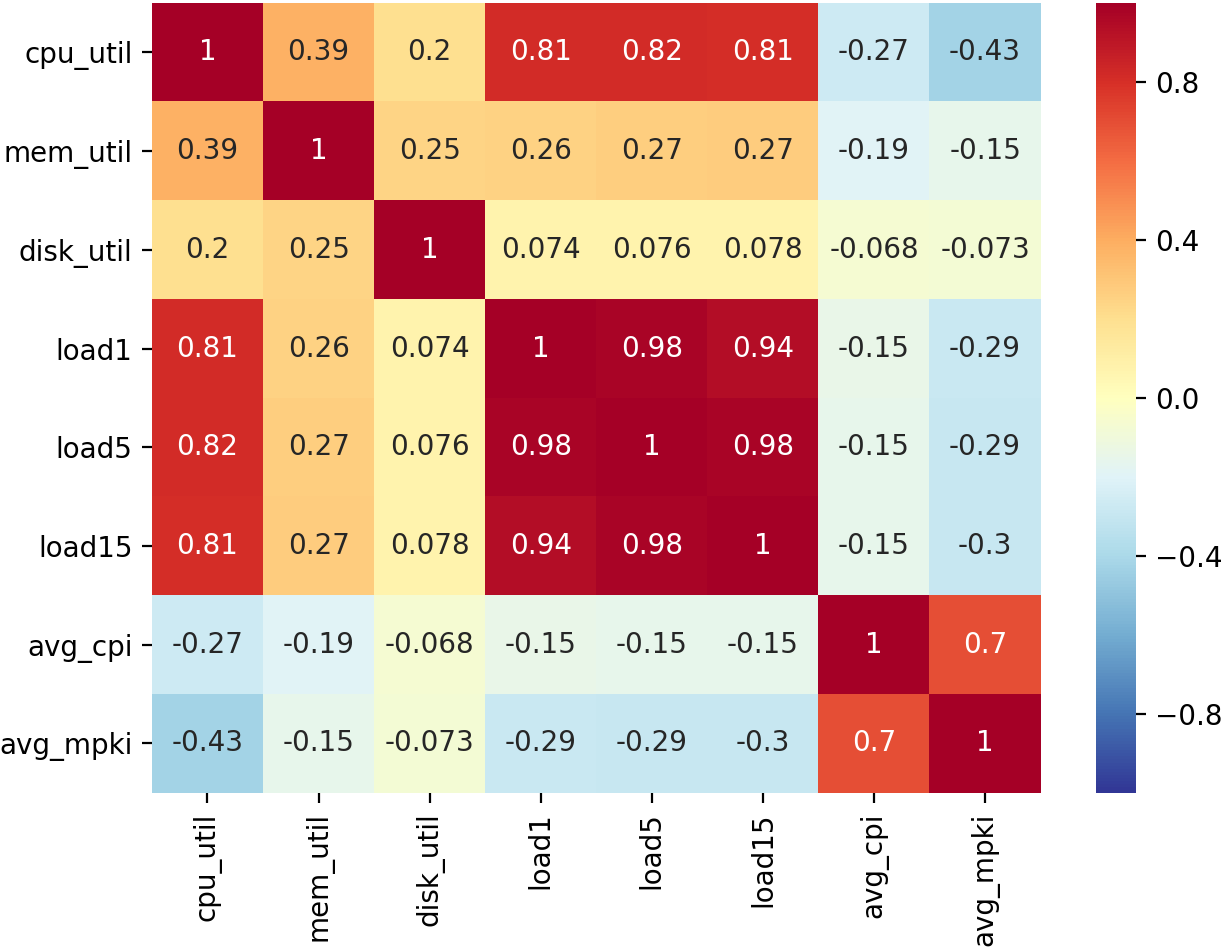
\includegraphics[width=.9\linewidth]{results/container_usage.png}
%   \caption{Latency-critical task's usage metrics}
%   \label{fig:container}
%  \end{subfigure}%
 
%   \begin{subfigure}[t!]{0.32\textwidth}
%   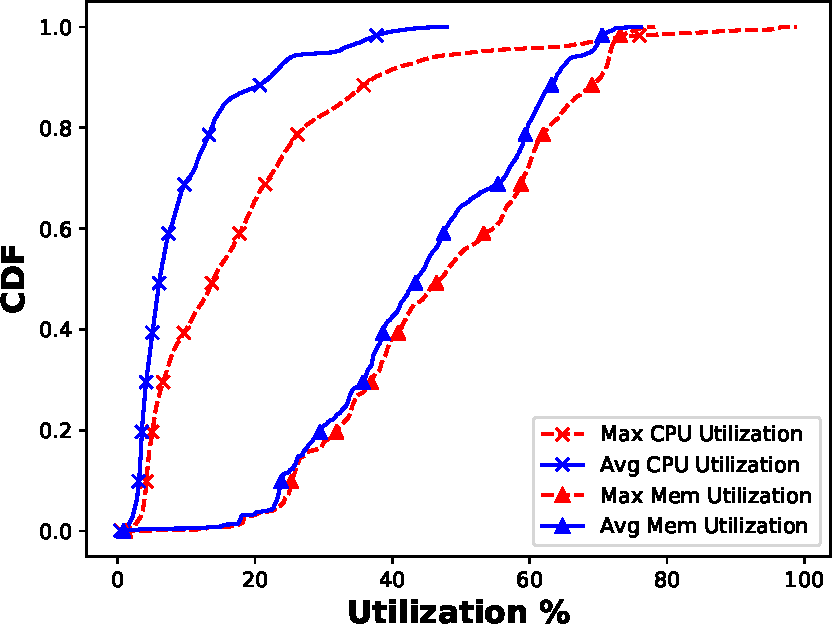
\includegraphics[width=.9\linewidth]{results/cdf.pdf}
%   \caption{Average \& Maximum CPU and memory utilization of latency-critical containerized production services.}
%   \label{fig:cont-mem}
% \end{subfigure}%

%   \begin{subfigure}[t!]{0.3\textwidth}
%   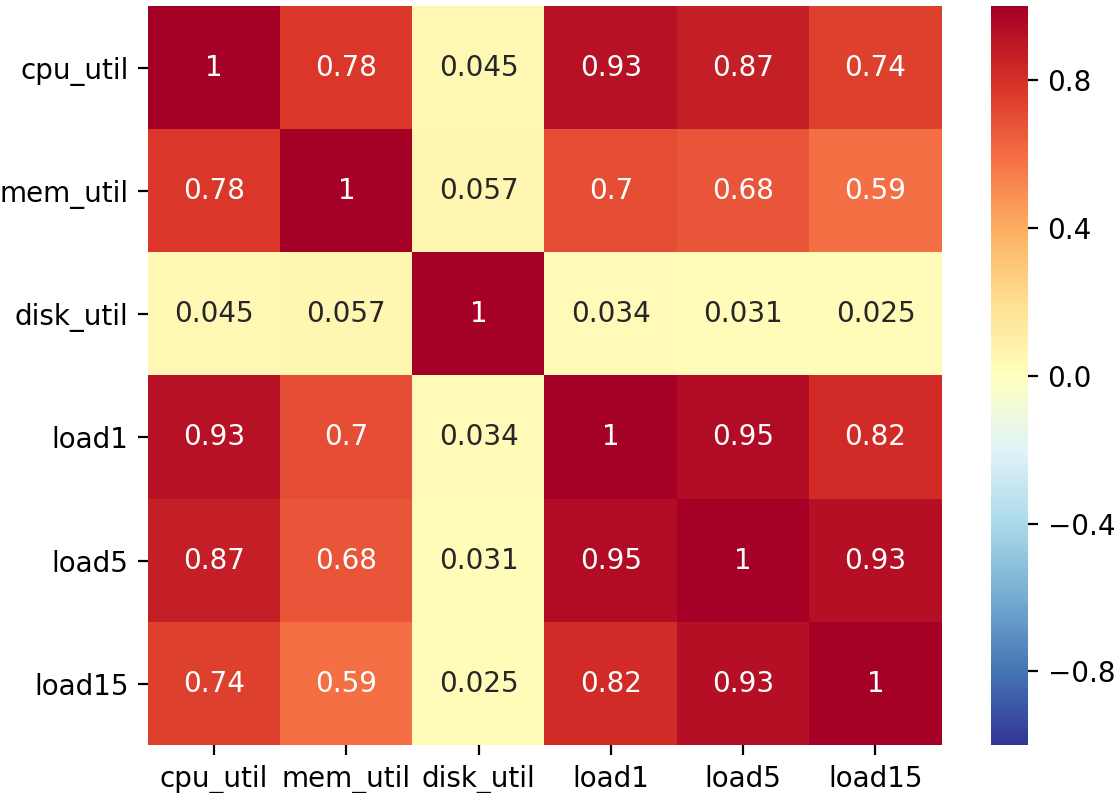
\includegraphics[width=.9\linewidth]{results/batch_usage.png}
%   \hspace{2mm}
%   \caption{Long running batch task's usage metrics}
%   \label{fig:batch}
% \end{subfigure}%
% \vspace{-2mm}
% \caption{Alibaba trace analysis of resource utilization of 1300 machines across 12,951 batch jobs \& 11,089 containers (12hr period).}
% \label{fig:ali}
% \end{figure*}

\begin{figure*}
\hspace{-10mm}
\begin{subfigure}[t!]{.42\textwidth}
  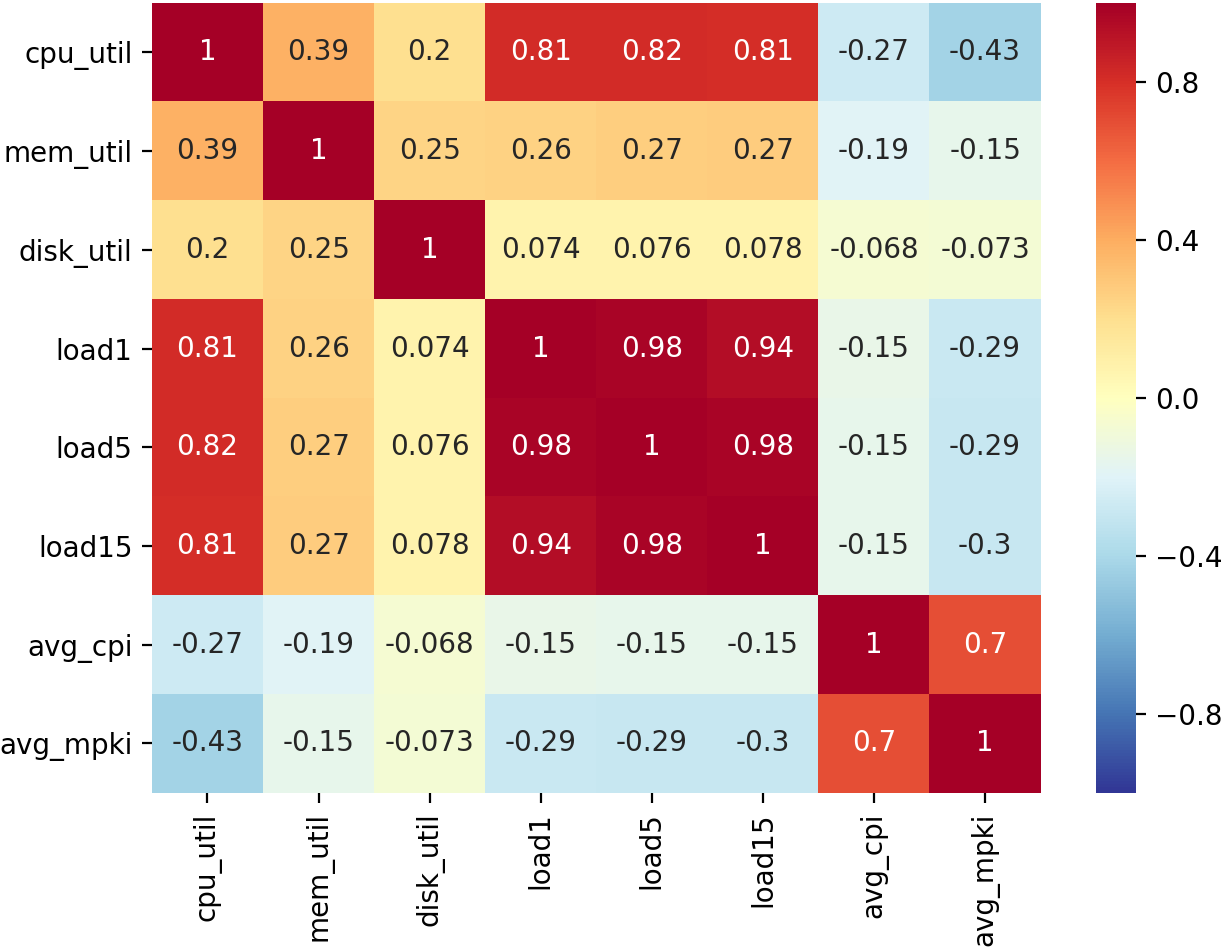
\includegraphics[width=.99\linewidth ,height=5.3cm, width=6.7cm]{results/container_usage.png}
  \caption{Latency-critical task's usage metrics}
  \label{fig:container}
 \end{subfigure}%
 \hspace{-5mm}
  \begin{subfigure}[t!]{0.3\textwidth}
  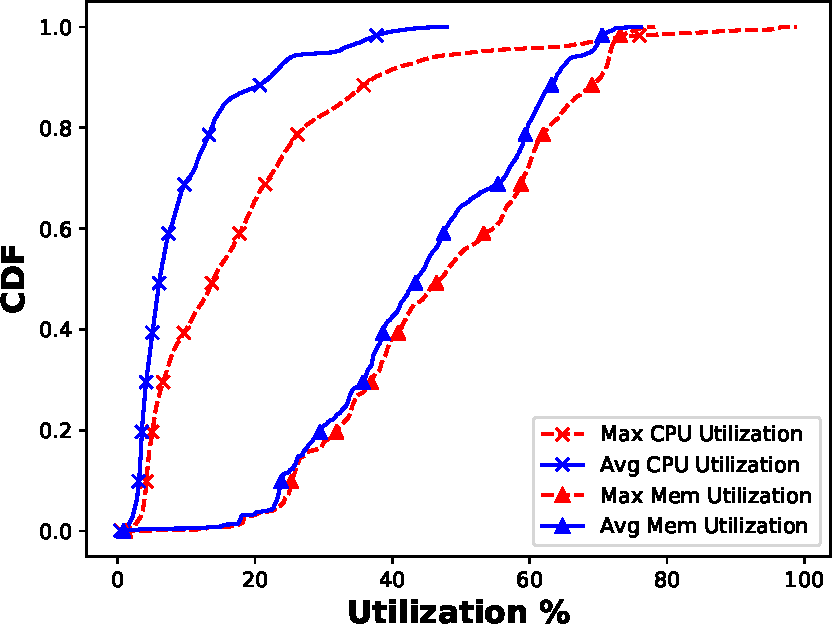
\includegraphics[width=.99\linewidth,height=4.5cm, width=5.3cm]{results/cdf.pdf}
  \caption{Average \& Maximum CPU and memory utilization of latency-critical containerized production services.}
  \label{fig:cont-mem}
\end{subfigure}%
  \begin{subfigure}[t!]{0.33\textwidth}

  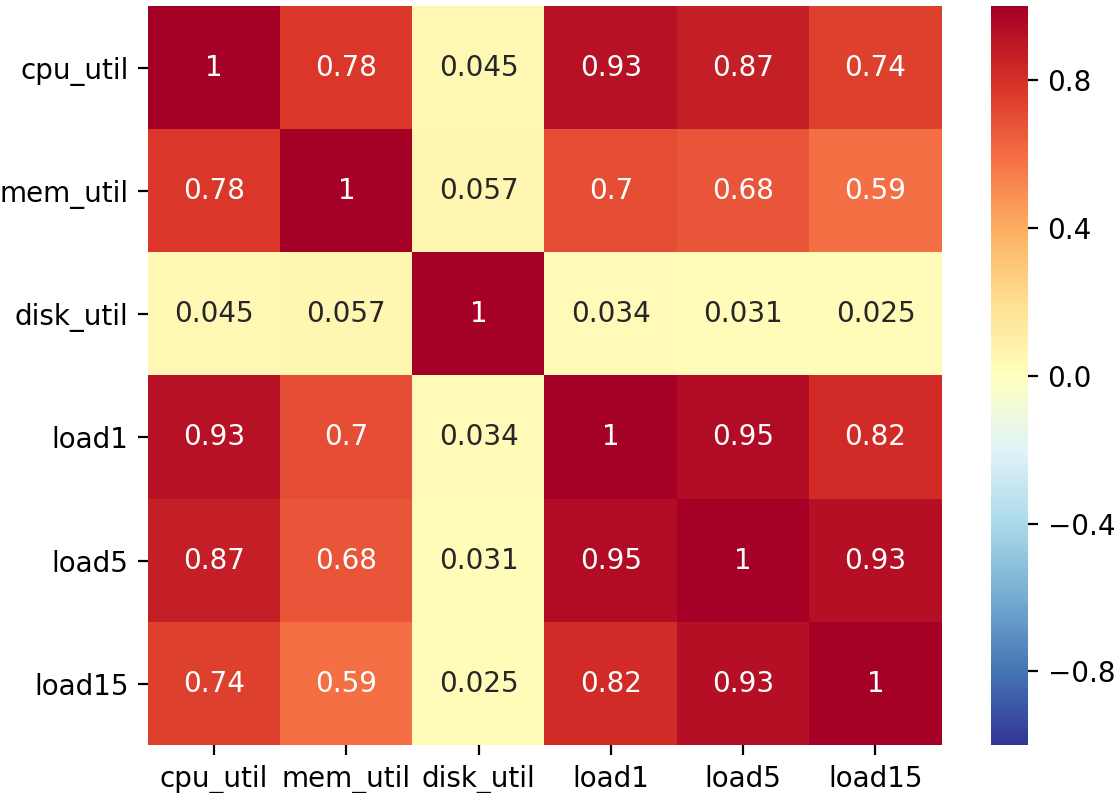
\includegraphics[width=.99\linewidth, height=4.8cm,width=6.4cm]{results/batch_usage.png}
  \hspace{2mm}
  \caption{Long running batch task's usage metrics}
  \label{fig:batch}
\end{subfigure}%
\vspace{-2mm}
\caption{Alibaba trace analysis of resource utilization of 1300 machines across 12,951 batch jobs \& 11,089 containers (12hr period).}
\label{fig:ali}
\end{figure*}

As a result, there is an inherent need for a GPU utilization-aware resource orchestration along with qos-aware job scheduler. In this paper, we propose \textit{Kube-Knots}\footnote{Google's \textit{Kubernetes} means helmsman or captain of the ship managing multiple containers. In \textit{Kubernetes},  \textit{Knots} orchestrates the scheduling speed of the accelerated containers.} by integrating \textit{Knots}, a GPU aware orchestration layer with \textit{Kubernetes}. Integrating \textit{Knots} with \textit{Kubernetes} enables GPU-aware resource orchestration used alongside with existing job schedulers to schedule for both CPU and GPU specific workloads. Since there is significant work done towards utilization aware CPU scheduling  \cite{Tang:2013:RRS:2451116.2451126,Marsbubbleup,Yang:bubbleflux}, in this paper, we focus only on scheduling for GPU specific workloads. Using \textit{Kube-Knots}, we make the following contributions:
\\
\begin{enumerate}[wide = 0pt, labelwidth = 1.3em, labelsep*=0em, itemindent = 0pt, leftmargin = \dimexpr\labelwidth + \labelsep\relax, noitemsep,topsep = 1ex, font=\normalfont]

\item \textit{Knots}, is a GPU resource orchestrator which works with a node-level GPU resource manager to monitor the real-time GPU utilization metrics at every node.

\item We generate datacenter representative GPU cluster workloads to evaluate our proposed schedulers on a ten node GPU cluster managed by \textit{Kubernetes} with \textit{Knots}.

\item We build three schedulers namely Resource Agnostic (Res-Ag), Correlation Based Prediction (CBP), and Peak Prediction (PP) that leverage the cluster-wide GPU utilization time-series data aggregated from \textit{Kube-Knots}.

%\item Cluster-wide GPU metrics are collected by the utilization aggregator at headnode, and the time-series data is used for future GPU scheduling decisions. Thus enabling \textit{Kube-Knots} to make GPU-utilization aware resource orchestration.

\item Our proposed CBP scheduler uses GPU usage correlation metrics to perform safe pod co-locations ensuring crash-free container resizing and efficient packing on GPUs.

\item CBP along with PP scheduler can guarantee the end-to-end QoS of latency critical queries by predicting loads of GPUs through ARIMA~\cite{arima} based time-series forecasting. This further reduces the QoS violations by up to 53\% when compared to the resource agnostic scheduler.

\item \textit{Kube-Knots}\footnote{We plan to release \textit{Kube-Knots} as an open-source plug-in patch for \textit{Kubernetes}, that could be leveraged by the community to dynamically orchestrate GPU-based containers via Kubernetes.} improves the cluster-wide GPU utilization through performance-aware workload consolidation by up to 80\%  for both 50$^{th}$ and 90$^{th}$ percentile utilization when compared to resource agnostic scheduler. Thus reducing the datacenter wide GPU energy consumption by 33\% on an average when compared against GPU agnostic orchestration.

\end{enumerate}


%------------------------------------------------------------------------------------------------------------------
\section{BACKGROUND AND MOTIVATION} 
\label{sec:motivation}
\subsection{Utilization vs Performance per Watt}
In traditional CPU-based datacenters, the optimum operating range is set and managed around 50-60\% core utilization across the datacenter. This is because the CPU processing elements are designed to operate for an average case load at peak energy efficiency~\cite{wong2016peak} in terms of performance per watt (PPW). Figure~\ref{fig:efficiency} plots the PPW of Memcached queries served by CPUs and GPUs, at different query load scenarios, where PPW is normalized with the PPW at 100\% load. For the CPU-bound queries, we observe that the peak energy efficiency at around 60\% to 70\% core utilization, but the PPW drops when utilization is further pushed by overclocking. We can see that the GPUs are fundamentally different from CPUs as their peak performance per watt is achieved only at 100\% load utilization of Streaming Multiprocessors (SMs). In case of Memcached-GPU~\cite{memcachedgpu} running individual queries are not energy proportional unless multiple queries are batched together. Batching multiple small queries is critical for energy efficiency while intuitively maximizing the throughput. However, operating the GPU at its peak energy efficiency and performance depends on the system scheduler's resource management policies.

\textbf{Design point 1:} \textit{Keeping the GPU utilization high is essential for high performance per watt.} 

\subsection{Cluster Workload Analysis}
In order to obtain very high utilization in GPUs, we need to know the application behavior in terms of resource request and usage trend. First, we focus on CPU specific workloads and later correlate the application behavior to GPU specific workloads. We analyze the recently open-sourced Alibaba production datacenter traces~\cite{baba} to gain insights into the nature of batch and latency critical jobs that are submitted to the CPU based datacenter and their corresponding resource consumption trends. Further, we investigate the inter-arrival times between these jobs to establish expected load at any given time for a production datacenter.

Alibaba's cluster traces were collected across 1300 CPU-based machines for a period of 12 hours at a granularity of every 60 seconds. We analyze both the batch and container workload behavior of 12,951 batch and 11,089 online service queries (containerized workload) in terms of their corresponding resource consumption trends. We summarize the following key observations: 

%There is a significant relationship between the cores, system load and memory resource consumption of latency-sensitive service jobs. Especially the system load recorded over the time are tightly correlated.
\begin{itemize}[wide, nosep, labelindent = 0pt, topsep = 0.3ex]
\item \textbf{Resource overcommitment - } Firstly, users tend to overstate their resource requirements. As observed from Figure~\ref{fig:cont-mem}, average CPU and memory utilization is 47\% and 76\% respectively. Half of the containers consume less than 45\% of the provisioned memory on an average. This over-consumption trend is also seen in CPUs, in which almost all the containers consume less than 50\% of the provisioned CPU cores. This is because, over-commitment indirectly helps to ensure the QoS of such queries by provisioning for the worst (peak) case. A cluster-wide resource orchestrator, while provisioning for an application, should not use the user-stated expected resource consumption as it leads to overall underutilization of the cluster. In case of CPUs, preemption and fine-grain resource sharing mitigates the problem, while it becomes a critical design point factor for a GPU scheduler. 

\textbf{Design Point 2:}\textit{ Due to varying resource needs of an application, instead of provisioning the resources for application's maximum utilization case, it is more resource efficient to provision for the average utilization case. It is ideal if the scheduler could dynamically provision and resize the containers based on the run-time growth of the application instead of static provisioning scheme.}\\

\item \textbf{Resource usage metrics are tightly correlated -}
Figure~\ref{fig:container} plots the Spearman's correlation across eight container resource utilization metrics as a heat map. Equation ~\ref{eqn:corr} gives the correlation score $\rho$ where, d$_{i}$ is the difference between the ranks (ordered in descending i.e, highest value gets rank 1 and lowest value gets rank 8) of corresponding utilization metrics in the heatmap and \textit{n} is the number of observations. Positive relationship between two metrics is represented by a score close to +1 and vice-versa. A score of 0.0 denotes that these metrics do not have any relationship. More positive the relationship, hotter is the color scheme (red). There is a significant relationship between the cores (core\_util), average system load recorded every second (load\_1) and memory resource consumption (mem\_util) of latency-sensitive service jobs. 
\end{itemize}
 \vspace{-1mm}
\begin{equation} 
\rho = 1-{}\frac{6 \Sigma d^{2}_i}{n(n^{2}-1)}
% r_{xy} = \frac{\sum x_i y_i - \sum x_i \sum y_i} {\sqrt{N \sum x_i^2 - (\sum x_i)^2} \sqrt{N \sum y_i^2 - \sum(y_i)^2}} 
\label{eqn:corr}
\vspace{-1mm}
\end{equation}

Figure~\ref{fig:batch} plots the correlation between six utilization metrics of batch workloads. It is seen that the memory utilization strongly correlates with the core utilization. Unlike latency sensitive queries, the batch applications exhibit strong correlation (both +vs \& -ve) between its utilization metrics. For example, the system load recorded over different sampling intervals, i.e. the Linux load average of the service instance usage at 1$^{st}$, 5$^{th}$and 15$^{th}$ second intervals, positively correlate with core utilization. On a similar note, CPU-utilization has a positive relationship with memory, but a negative relationship with the last level cache misses per kilo instructions (MPKI). This is a common trend across the workload.

This pair-wise correlation plot provides insights about latency sensitive application's resource usage behavior and the corresponding intertwined relationships across different resource usage metrics. It can be seen that the scheduler provisions for the dominant resource consumption (i.e., type of resource that is highly utilized)~\cite{Ghodsi:2011:DRF:1972457.1972490}. In case of co-located applications, the dominant resource type should not be the same. For example, co-locating a CPU bound application with a similar application would lead to severe SLA violations. 

\textbf{Design Point 3:}\textit{ Correlation between different resource utilization metrics need to be considered during placement to guarantee the performance of the scheduled application.}


% The production system scheduling policies are designed and optimized for CPUs and overlook accelerators like GPUs. We identify several GPU-based datacenter design choice issues and challenges below. 

 

\begin{figure}
\centering
  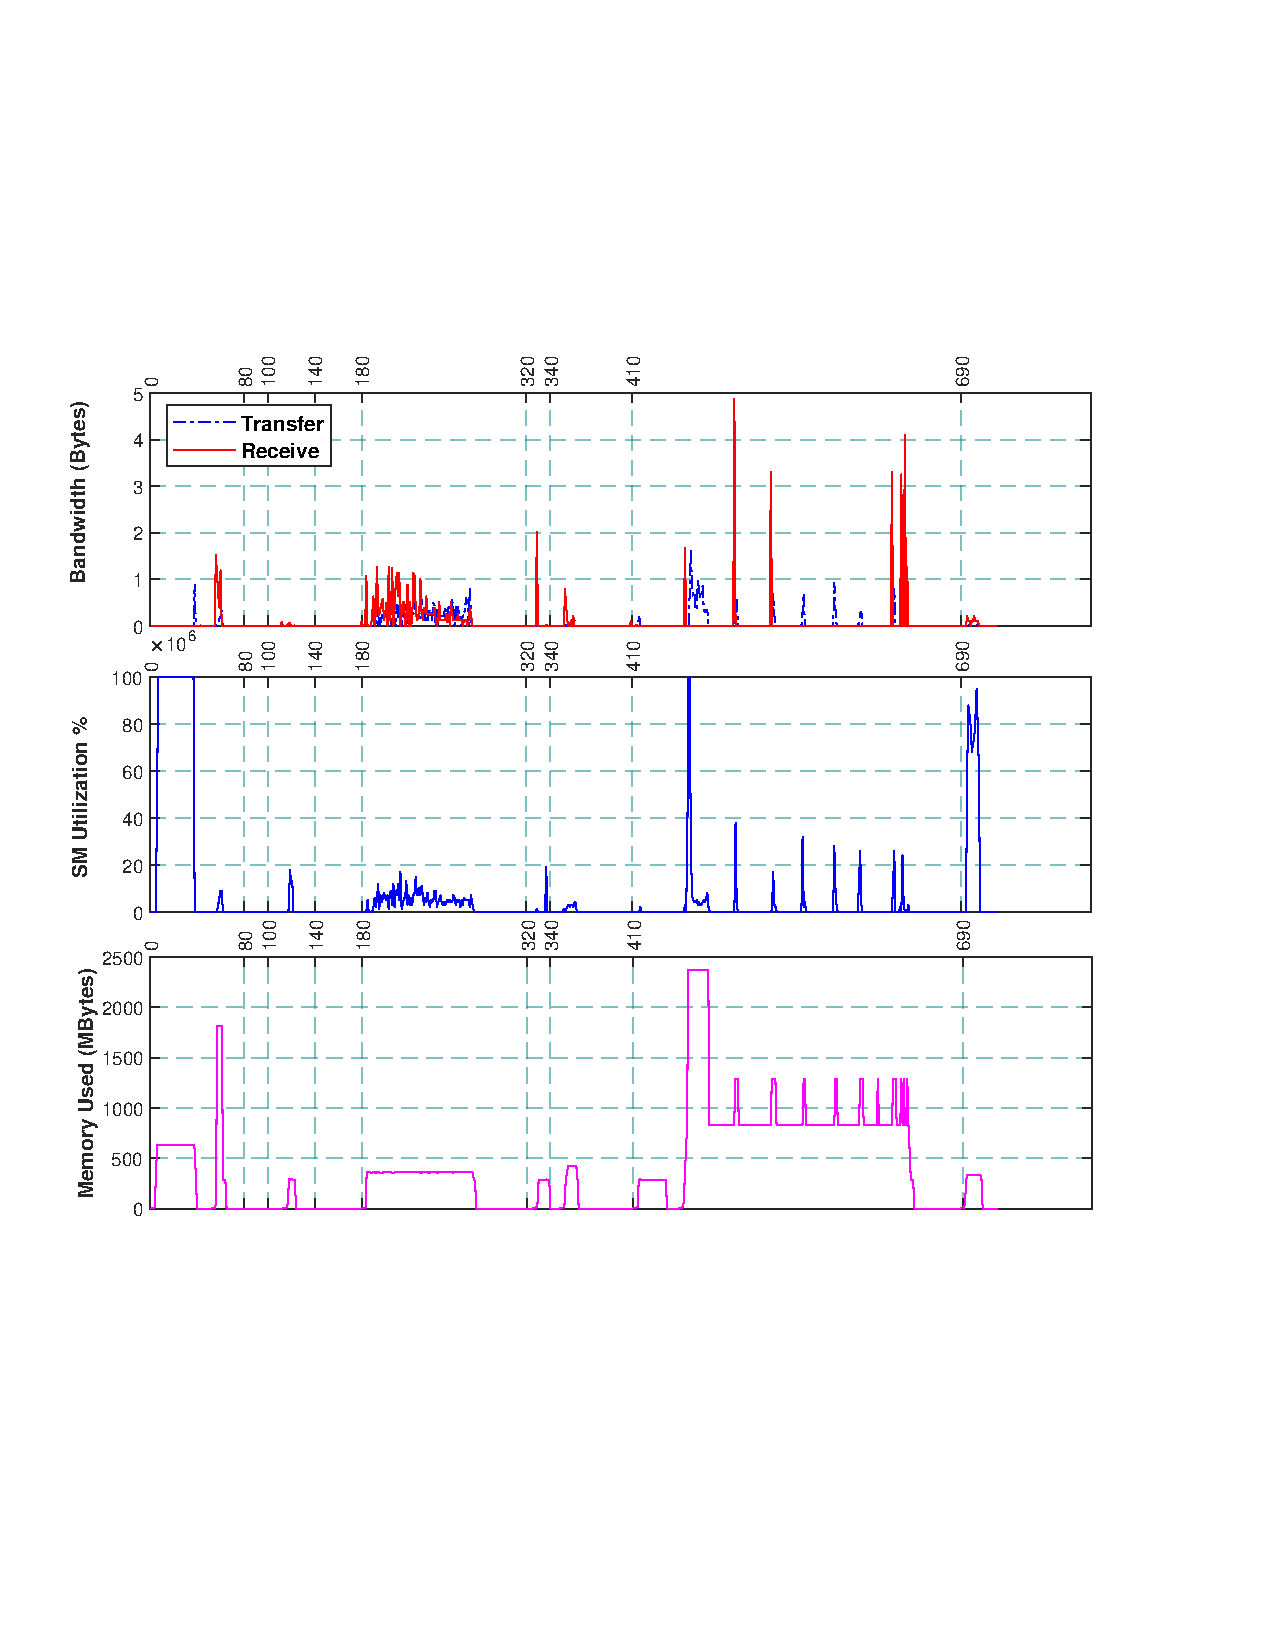
\includegraphics[width=0.99\linewidth ]
  {results/util.pdf}
  \vspace{-2mm}
  \caption{GPU Resource consumption of entire Rodinia suite on Nvidia's P100 GPU. The grid-lines mark the individual benchmark's runtime.(where x-axis is time in milliseconds)}
  \label{fig:rodinia-peaks}
\end{figure}



\subsection{GPU Workload Characterization}
We analyzed the resource consumption trends of both latency sensitive and batch workloads in Alibaba's production datacenter, which have correlating utilization metrics with respect to CPU, memory, disk, load, etc. Further, we apply this resource consumption trend to extend it to represent a GPU-based datacenter load and job inter-arrival scenario. To this end, we identified popular production workloads which subscribe to GPUs. Recall that GPU-based cloud services are becoming ubiquitous with the advent of Machine Learning as a Service (MLaaS)~\cite{gujarati2017swayam}. There have been significant industry-wide efforts on accelerating these queries through compute-intensive libraries such as cuDNN~\cite{ChetlurWVCTCS14}. These libraries are similar to MPI collective operations like broadcast, scatter-gather, all reduce, etc., and are specifically optimized for GPU data flow. 

The workloads use high-level libraries like Tensorflow, which are hosted as micro-service deployments as containers and are shipped via container orchestrators like Kubernetes~\cite{kubernetes}, Mesosphere~\cite{mesosp}, Docker swarm~\cite{swarm}, etc. Generally, these deployments are hosted as services such as object detection, feature extraction, etc. Queries to these containers arrive in short bursts, and the containers are also short-lived. For example, the average image recognition DNN-based inference query takes 90\textit{ms} on Nvidia P100 \cite{nvidia-dnn} whereas other batch jobs may run on a GPU for hours like an HPC application or even Proof-of-Work (PoW) for block-chain based crypto-currency mining.
%\subsection{Memory Fragmentation in Application Frameworks}
In order to create a representative workload mix for GPUs, which consists of both batch workloads and user-facing queries: (i) we use applications from Rodinia workload suite \cite{che2009rodinia} to mimic typical GPU bound HPC and compute-intensive workload submitted to the datacenters and, (ii) we use a mix of DNN based inference queries from Djinn and Tonic workload suite for user facing queries. \cite{hauswald2015djinn}. We execute each application from the workload on single GPU node to understand the batch-workload's resource demands. The details of the node are described in Table \ref{tbl:hw-config}. More details about the workload are explained further in Section \ref{sec:modeling}.

% \textbf{Design point 4:}\textit{ Ensuring the Quality of Service in case of applications that have stricter deadlines is an onus on the job scheduler.} 

\subsubsection{GPU Batch Workload}
Figure~\ref{fig:rodinia-peaks} plots different GPU resource consumptions over time for the eight different applications, which were run sequentially. We characterize memory used, Streaming Multiprocessor (SM) utilization and PCIe bandwidth which are three dominant resources for a batch application. It is observed that most of the applications could be co-located with one another since the resource consumption is relatively low. From Figure \ref{fig:rodinia-peaks}, we observe that the resource consumption of applications may not always peak at the same time. This temporal nature of the application resource usage can be exploited to avoid resource capacity violations, while sharing the resource. Further, we observe that these applications show a very deterministic pattern of phase changes. For example, typically if an application's input bandwidth activity is high, it is implied that the compute and memory would follow the same trend in near future. These subtle utilization cues could be picked up through real-time feedback and can be applied while making scheduling decisions. 

\textbf{Design point 4:} \textit{Batch application's utilization footprint is fairly predictable across the application's lifetime.}
% \vspace{-0.2in}
\subsubsection{GPU User-Facing Queries}
\label{sec:TF-mem-sec}
The Djinn and Tonic workload uses Tensorflow as its DNN application framework. TensorFlow(TF) not only provides the framework for executing ML queries but, also manages the execution flow of the query that run inside GPU. By default, TF earmarks the entire GPU memory despite actual workload demands. The TF runtime is designed to make this a default choice because GPUs are assumed to run a single context and not designed for multi tenant/application scenarios. In public datacenters to keep the operating costs low, it is ideal to share the GPUs because the individual application/tenant utilization is generally low. 

Figure~\ref{fig:tf-frag} shows the maximum memory consumption of different machine learning inferences. For most of the single inference queries, the memory consumption is less than 10\%. We batched these queries up to 128 queries per batch request, however, the majority of the inferences even with batching consume less than 50\% of the device memory. Whereas if the same application with the TF  application framework, they always earmark 99\% of the GPU memory causing severe internal memory fragmentation. This is a common case of resource overstatement from the workload behavior that we observed across Alibaba traces as explained in section \ref{sec:motivation}. 
% We do not consider SM utilization and PCIe bandwidth as they are not correlating as explained in Figure ~\ref{fig:container}. 
% When these inferences run inside TF-managed GPU, by default, the entire device memory is statically allocated for these inferences despite the actual consumption. 

Application frameworks like TF would always GPU resources by default leading to internal memory fragmentation. This directly affects the scheduler's global policies for fairness and performance. It is ideal for a datacenter scheduler to have two essential properties, namely, sharing incentive and strategy proofness~\cite{Ghodsi:2011:DRF:1972457.1972490}. In this case, neither can be ensured because the cluster-level resource manager has no control over the GPU device. In order to pack more applications to increase the utilization, the applications have to be provisioned by the datacenter scheduler by knowing the real-time GPU utilization metrics. 

\textbf{Design point 5:} \textit{It is essential to expose the application framework APIs to the job scheduler to avoid internal resource fragmentation.}

\begin{figure}
  \centering
  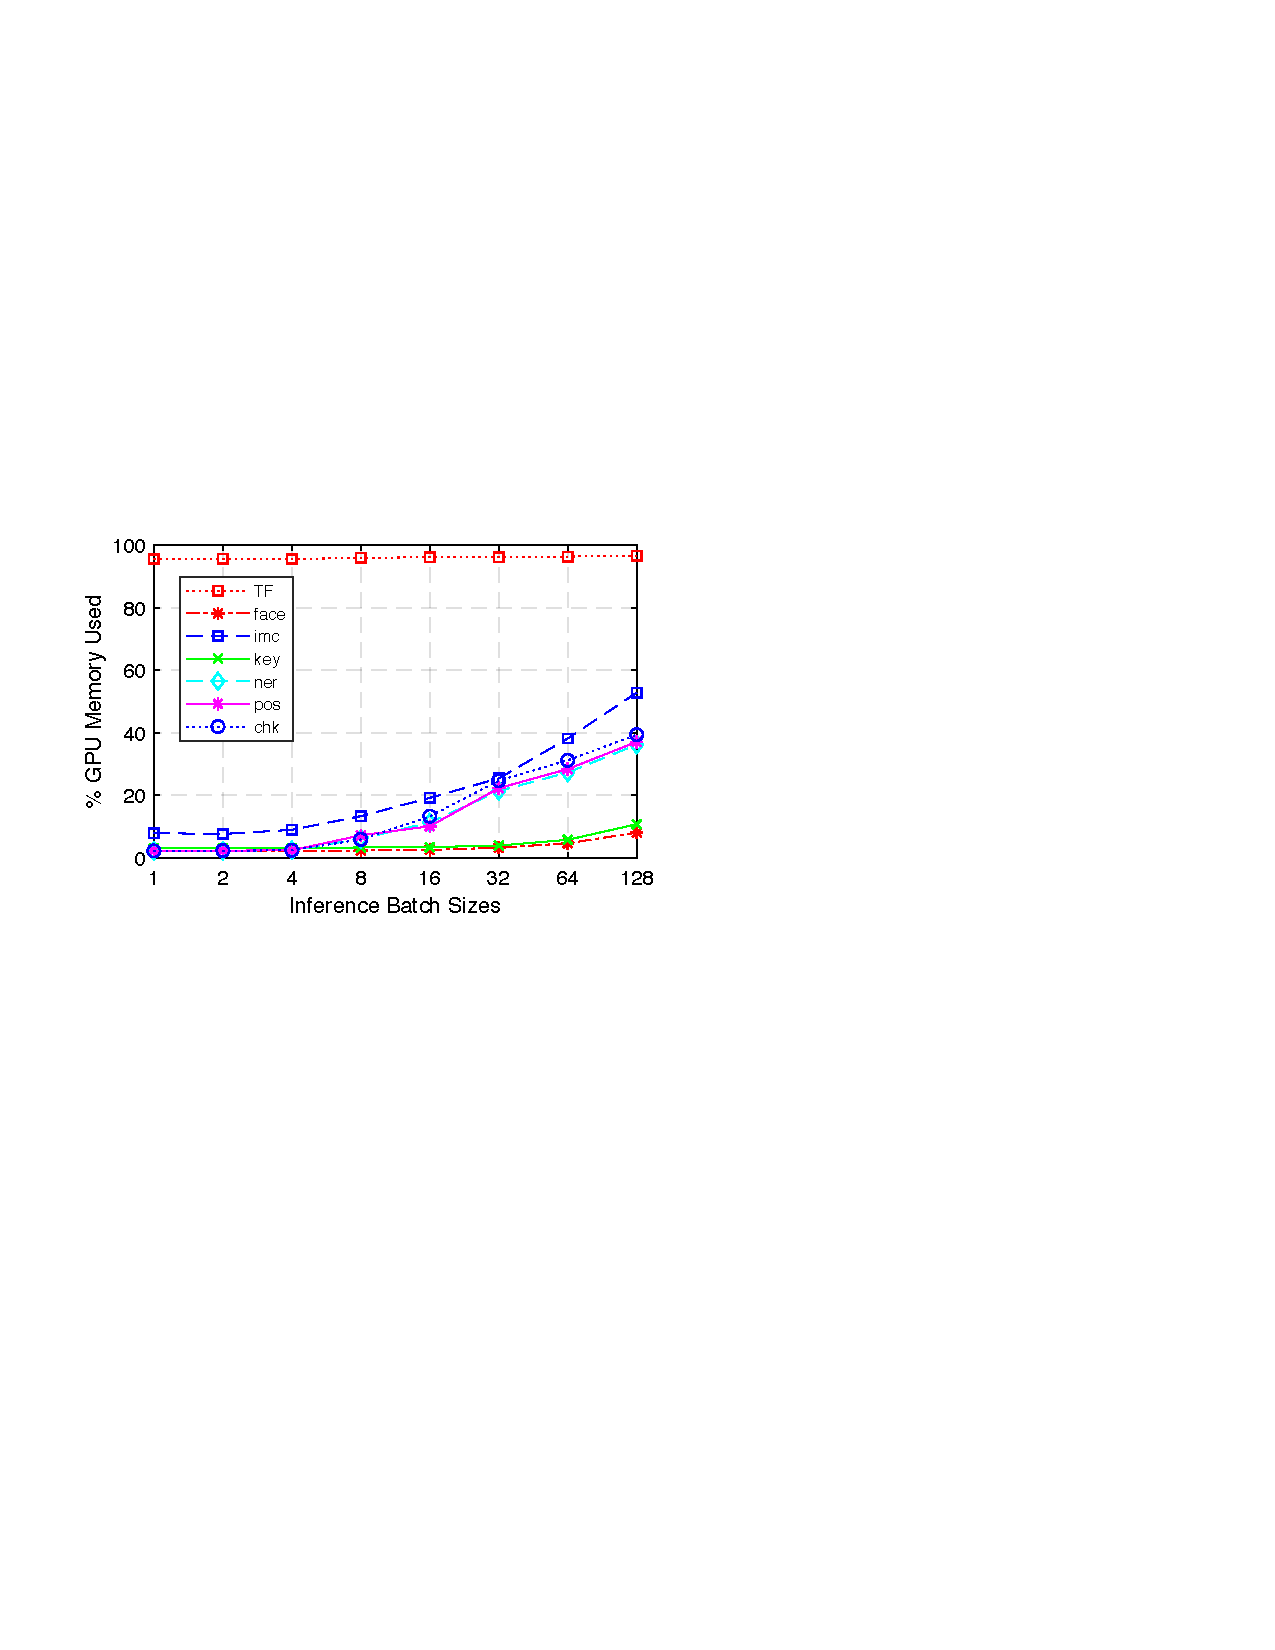
\includegraphics[width=.9\linewidth]{results/mem-fragmentation.pdf}
  \vspace{-2mm}
  \caption{Internal memory fragmentation of DNN inferences of Djinn and Tonic workload suite. TF is the Tensorflow managed memory consumption}
  \label{fig:tf-frag}
\end{figure}

% \item \textbf{Conservative scheduling policies -} 
% This results in a heavy imbalance of resource consumption trends, and it leads to resource fragmentation and poor energy efficiencies.
% \end{itemize}

% CPU systems are fairly resilient to these policies and overcome these challenges by resource virtualization, preemption, and load balancing. However, GPUs lack such support; therefore, CPU based resource orchestration and scheduling techniques cannot be applied to accelerators.


%%%%%%%%%Commented for space%%%%%%%%%%%%%%%%%%%%%%


% \vspace{-0.1in}
% \subsection{GPU Orchestration Challenges}
% Next, we explore the potential problems which will be encountered when both batch and user-facing queries are scheduled to the GPU concurrently. Although there are industry-wide efforts to support preemption of GPU kernels, still the technique is primitive and lacking when compared to CPUs. For example, when a batch task is scheduled on a GPU, the latency sensitive queries scheduled to the same node incur severe queuing delays and these kernels cannot be prioritized or run until the batch task finishes. By default, the uniform scheduler of Kubernetes is designed based on the fact that the GPUs are not shared across multiple containers. Therefore, ensuring QoS is entirely dependent on container startup latencies and queuing delays. The former could be mitigated by scheduling to a node which already has the container image. However, queuing delay is determined by both the kernels (apps) that currently are using the resources and the ones that are already ahead in the queue. Length of the queue can be a static indicator but however, just that would not suffice to guarantee the application turnaround time. Hence, real-time resource utilization feedback is an important metric for a scheduler to make effective orchestration decisions. Further, we do not make any changes to the application framework scheduler (tensorflow DAG scheduler) rather we augment \textit{Knots}, a GPU aware orchestration layer, to Kubernetes and design three scheduling schemes which leverage \textit{Knots}. 



%We discuss the challenges and how they are addressed in Section \ref{sec:modeling}. 

%\textbf{Design Point 6:}\textit{ GPU resource utilization metrics are critical to ensure the QoS of a particular application especially when they are co-located. An effective GPU resource scheduler would need to be dynamic and utilization aware.}

% To this end, as shown in Figure~\ref{fig:kubeknots}, we integrate {Knots}, an accelerator-aware orchestration layer with \textit{Kubernetes} which overcomes the above-listed challenges and enables cluster-wide GPU scheduling with end-to-end performance guarantees.

%%------------------------------------------------------------------------------------------------------------------
\section{KNOTS DESIGN AND INTEGRATION} 
\label{sec:modeling}

% However, this does not guarantee the QoS of latency sensitive queries because of reasons such as resource interference and application scaling characteristics as discussed in Section \ref{sec:motivation}

Motivated by our five key observations for a robust GPU-aware orchestration layer, we built \textit{Knots} and integrate it with \textit{Kubernetes} enabling GPU-aware orchestration.

\subsection{Knots Design}
Recall that, in order to make an effective scheduling decision at the cluster-level for a heterogeneous cluster with GPUs, \textit{Kubernetes} needs to know the real-time utilization of the accelerator devices to schedule to a node that would guarantee the end-to-end container performance. To ensure this, we design \textit{Knots} to collect and log the real-time GPU utilization metrics through pyNVML~\cite{pynvml}, which is a Python-based API library that exposes utilization metrics to the node-level aggregator. As shown in Figure~\ref{fig:kubeknots}, we log the following five GPU metrics in real-time: (i) streaming multiprocessor (SM) utilization, (ii) memory utilization, (iii) power consumption, (iv)transfer bandwidth and, (v) receive bandwidth . These metrics are pushed to a node-level Influx-DB (IDB) \cite{InfluxDB} time-series database. \textit{Knots} in the head node can query the GPU nodes for utilization data via the utilization aggregator which is further explained in detail in Section \ref{sec:scheme}. The frequency at which the \textit{Knots} queries the IDB, determines the prediction accuracy and the quality of scheduling. When the pod is scheduled to the respective node, it pulls the docker image of the pod from a centralized docker image hub. From section~\ref{sec:TF-mem-sec}, we infer that memory utilization is a crucial metric, which \textit{Knots} leverages for container resizing and capacity provisioning. However, the other metrics like SM Utilization and I/O bandwidth are also used by the schedulers built leveraging \textit{Knots} discussed in further sections. 

\subsection{Representative GPU workload}
We next describe a representative workload that we use to capture the GPU context correctly. Since accelerators like GPUs in production datacenters are relatively recent, we wanted to faithfully capture the dynamics of applications that would be representative of a production datacenter load. As discussed in Section \ref{sec:motivation}, we choose eight scientific applications from the Rodinia benchmark suite~\cite{che2009rodinia} to represent the datacenter batch jobs. For user-facing services, we used a mix of DNN-based inference queries from Djinn and Tonic workload suite~\cite{hauswald2015djinn} (refer Table~\ref{tbl:appmix} \footnote{The abbreviations for application names can be found in \cite{hauswald2015djinn}}). 

We did initial performance characterization experiments to determine the performance demands to come up with three different bins based on load and covariance as shown in the Table~\ref{tbl:appmix}. As observed earlier from Figure \ref{fig:rodinia-peaks}, a batch application can subscribe to highly correlatable GPU resources such as SM, memory, and bandwidth. (e.g., at time quantum 450, all the three resources are highly utilized which is classified as HIGH load). We repeatedly schedule the same set of workloads within a bin and start logging the performance metrics once a steady state is achieved.  We co-locate both the batch and production jobs on ten nodes which have an Nvidia P100 GPU. These GPUs are attached to their respective CPU hosts, and the queries are scheduled from a head node (configuration details in Table~\ref{tbl:hw-config}).

\begin{figure}
  \centering
  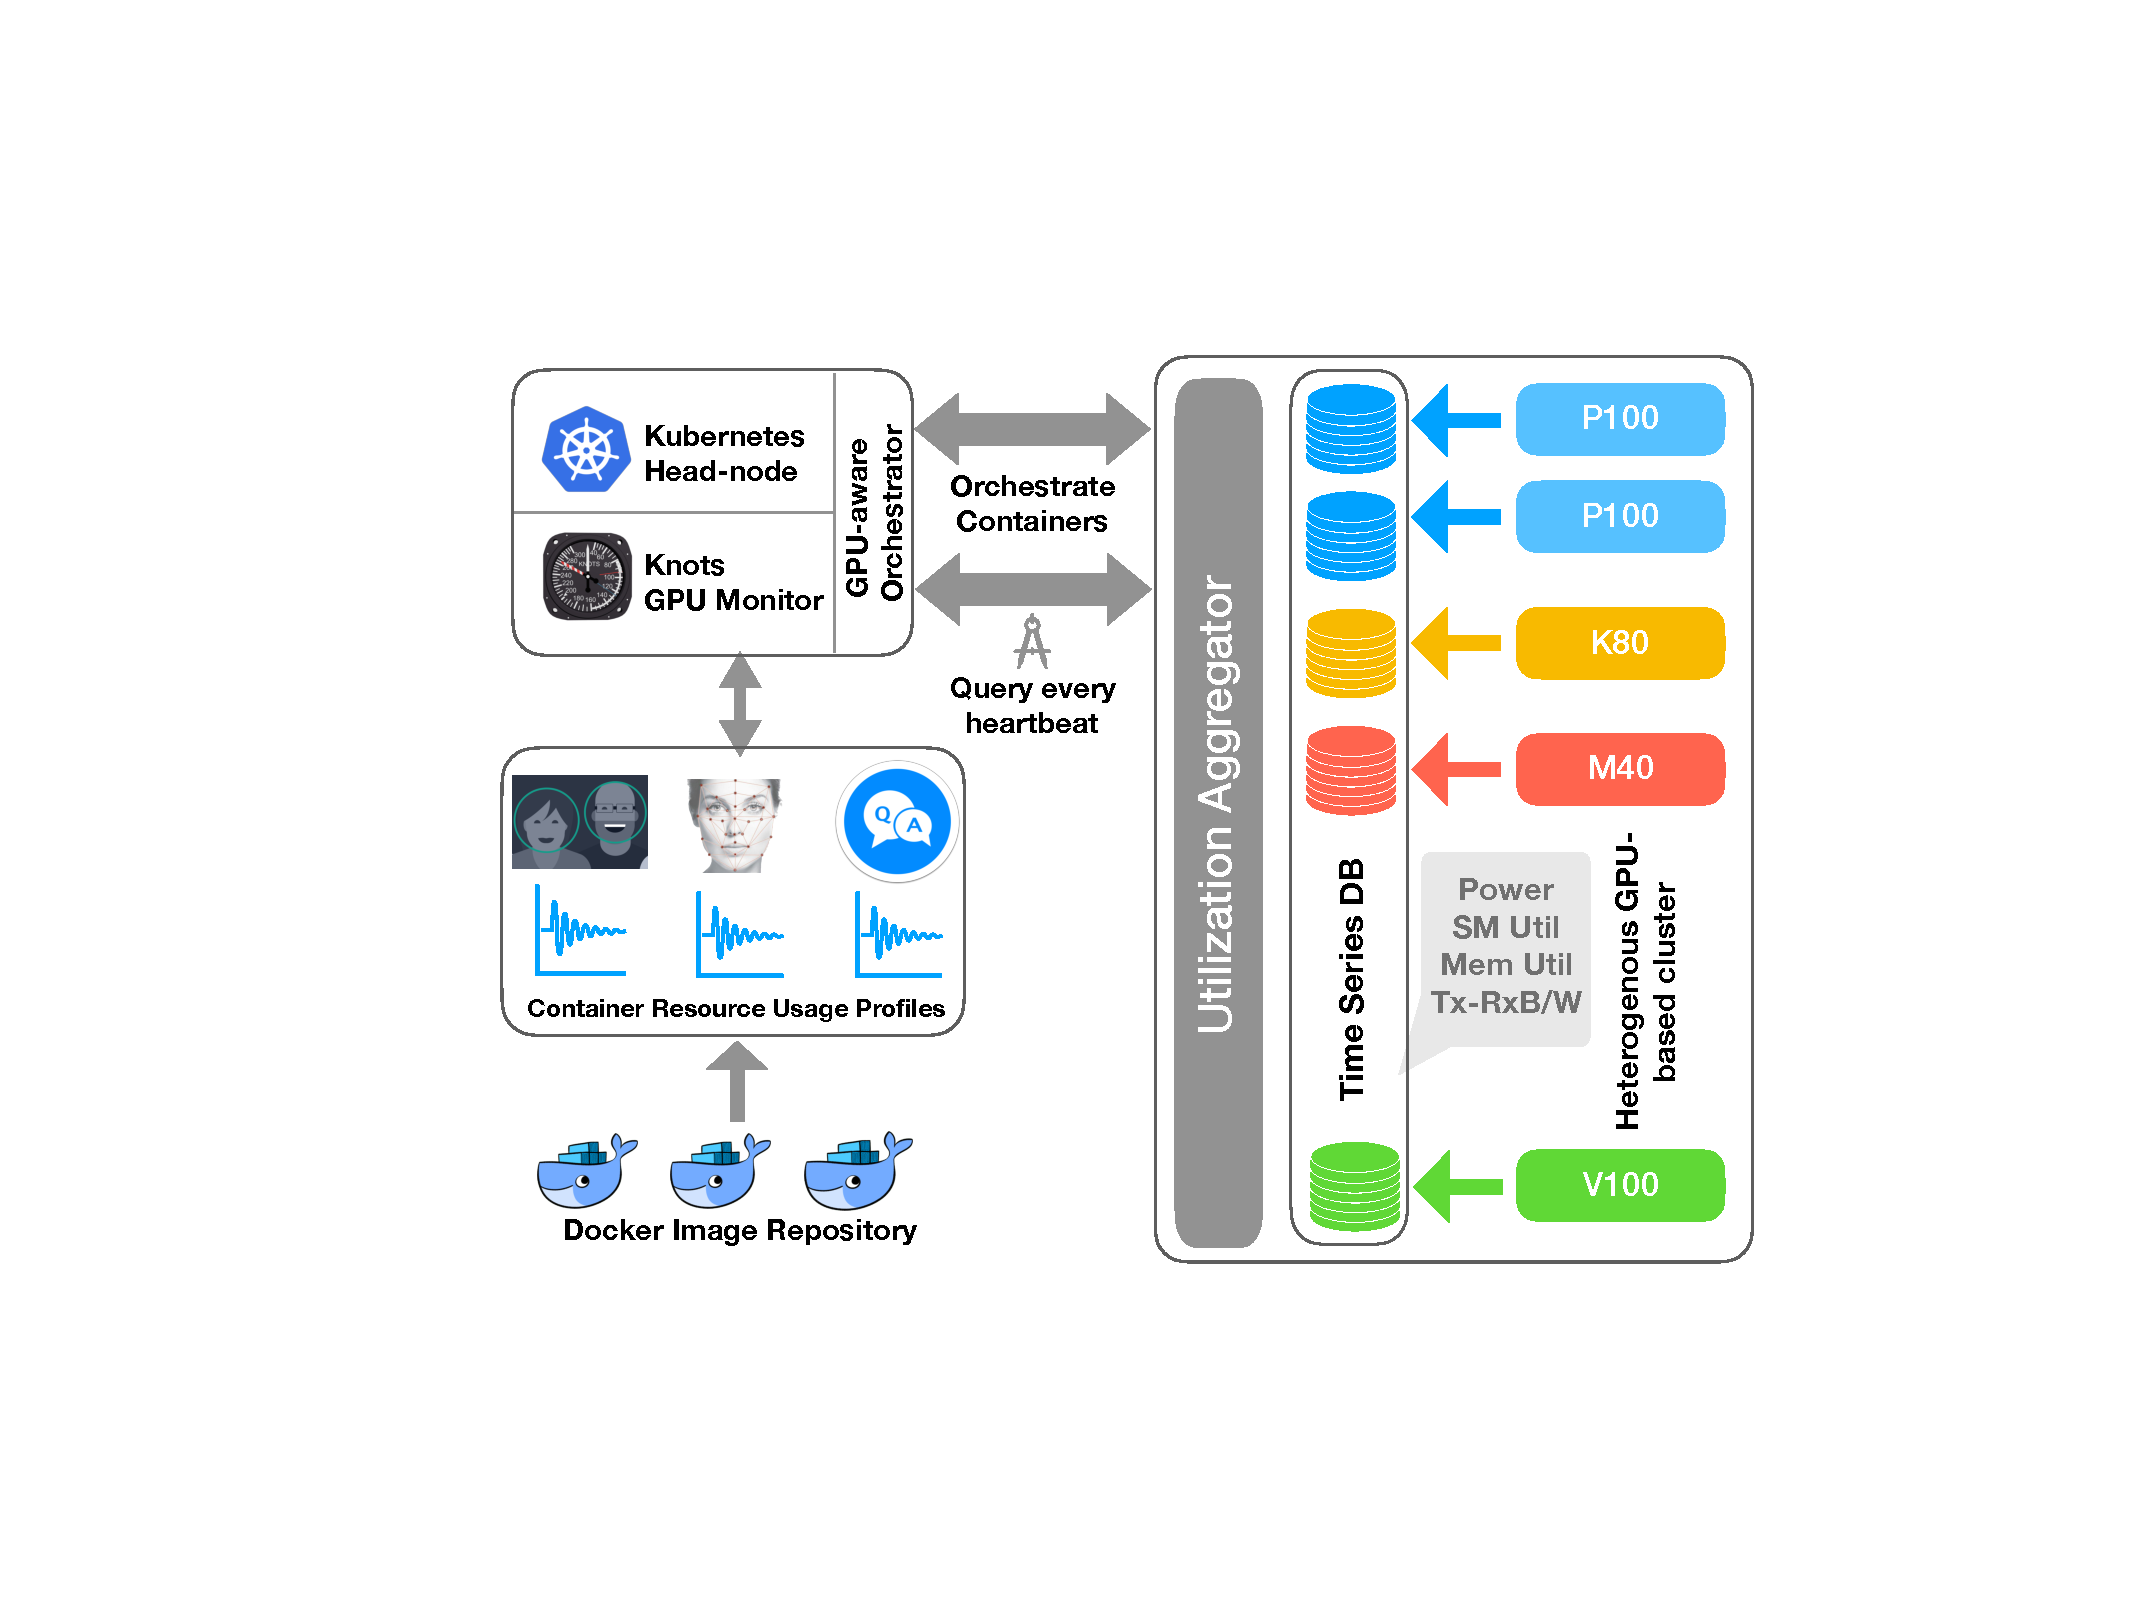
\includegraphics[width=.99\linewidth]{results/kube-knots.pdf}
  \caption{\textit{Kube-Knots} GPU orchestrator design.}
  \label{fig:kubeknots}
\end{figure}

% \vspace{-0.1in}
% \begin{center}
% \textit{The more you know about the past, the better prepared you are for the future - T. Roosevelt}
% \end{center}

\begin{table}[t]
%\setlength\extrarowheight{5pt}
% \begin{center}
\begin{minipage}{.99\linewidth}
\setlength\tabcolsep{1.1pt}
\resizebox{\textwidth}{!}{%
\renewcommand{\arraystretch}{1.2}
 \begin{tabular}{||c | c | c | c |c | c | c | c |c||} 
 \hline
 %\multicolumn{8}{|c|}{GPU Cluster Workload Mix} \\
 %\hline\hline
 \multicolumn{5}{|c|}{Batch workloads from Rodinia suite}&{Latency critical}&{Load}&{COV}\\
  \hline
  App-Mix-1 & leukocyte & heartwall & particlefilter & mummergpu & face,key & HIGH & LOW\\
 \hline
 App-Mix-2 & pathfinder & lud & kmeans & streamcluster & chl,ner,pos & MED & MED\\ 
 \hline
 App-Mix-3 & particlefilter & streamcluster & lud & myocyte & imc,face  & LOW & HIGH\\  
  \hline
\end{tabular}}
% \end{center}

\caption{GPU load and covariance for cluster workload suite mixed with batch jobs and latency critical ML inference queries.}
\vspace{-5mm}
\label{tbl:appmix}
\end{minipage}
\end{table}


\begin{figure*}[!tbp]
\begin{subfigure}[b]{0.33\textwidth}
  \centering
  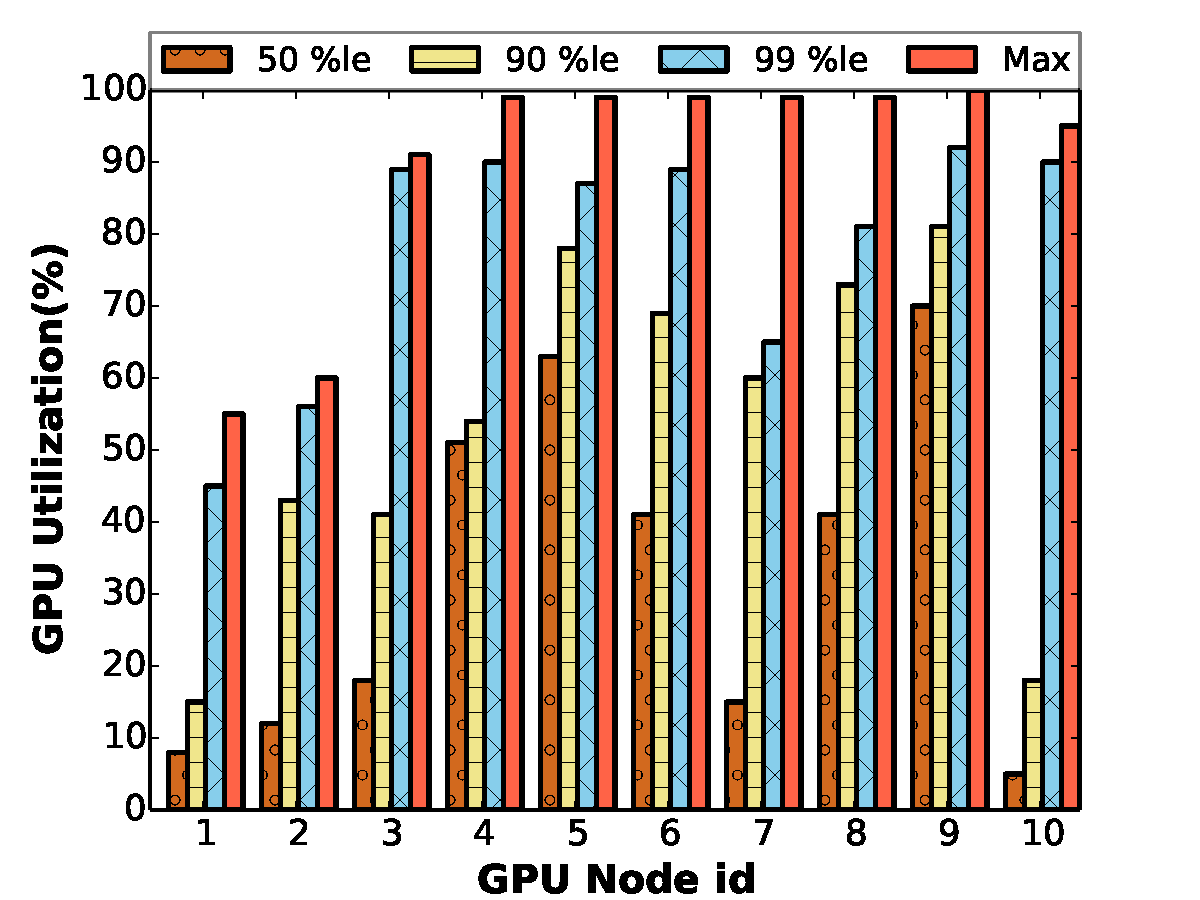
\includegraphics[width=1.1\linewidth]{results/app1-high.pdf}
  \caption{Application-Mix-1}
  \label{fig:app1}
\end{subfigure}
\begin{subfigure}[b]{.33\textwidth}
  \centering
  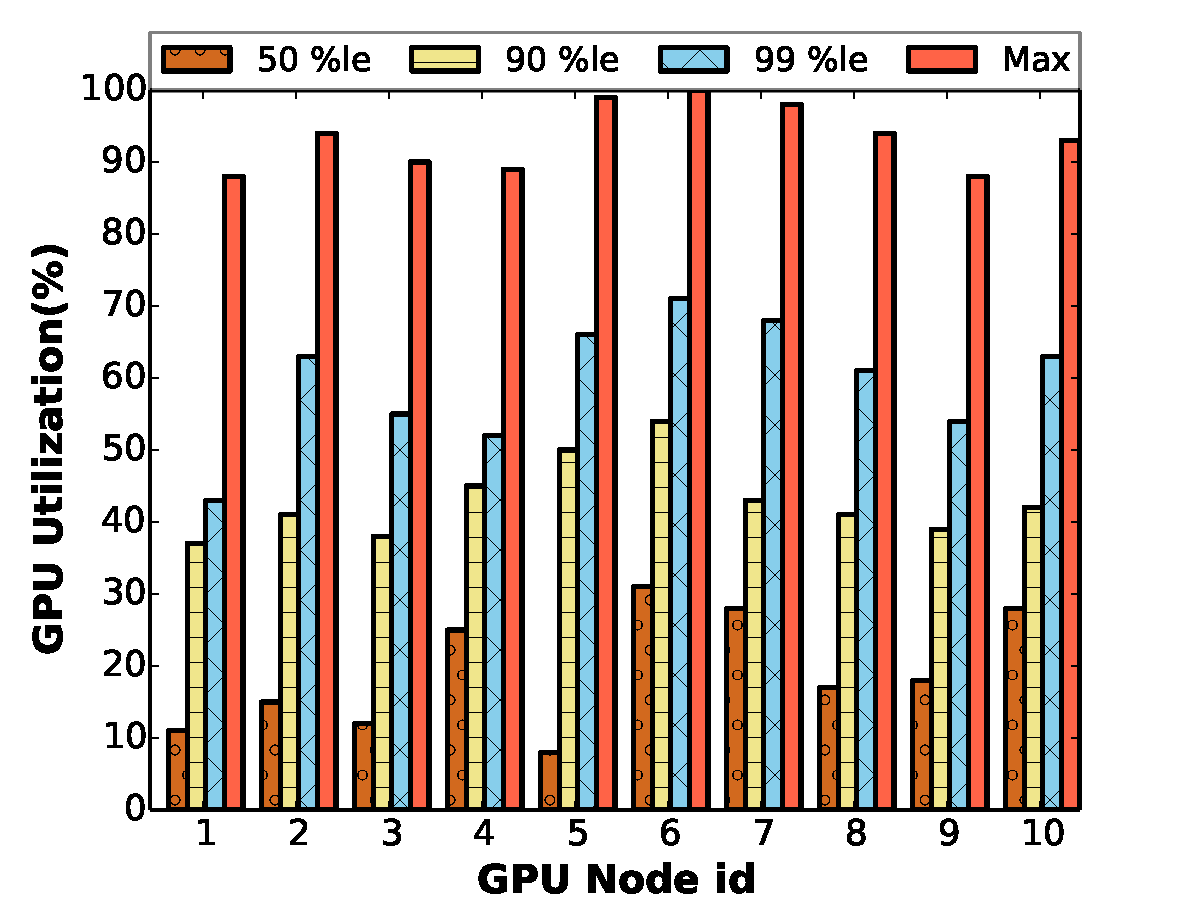
\includegraphics[width=1.1\linewidth]{results/app2-med.pdf}
  \caption{Application-Mix-2}
  \label{fig:app2}
\end{subfigure}
\begin{subfigure}[b]{.33\textwidth}
  \centering
  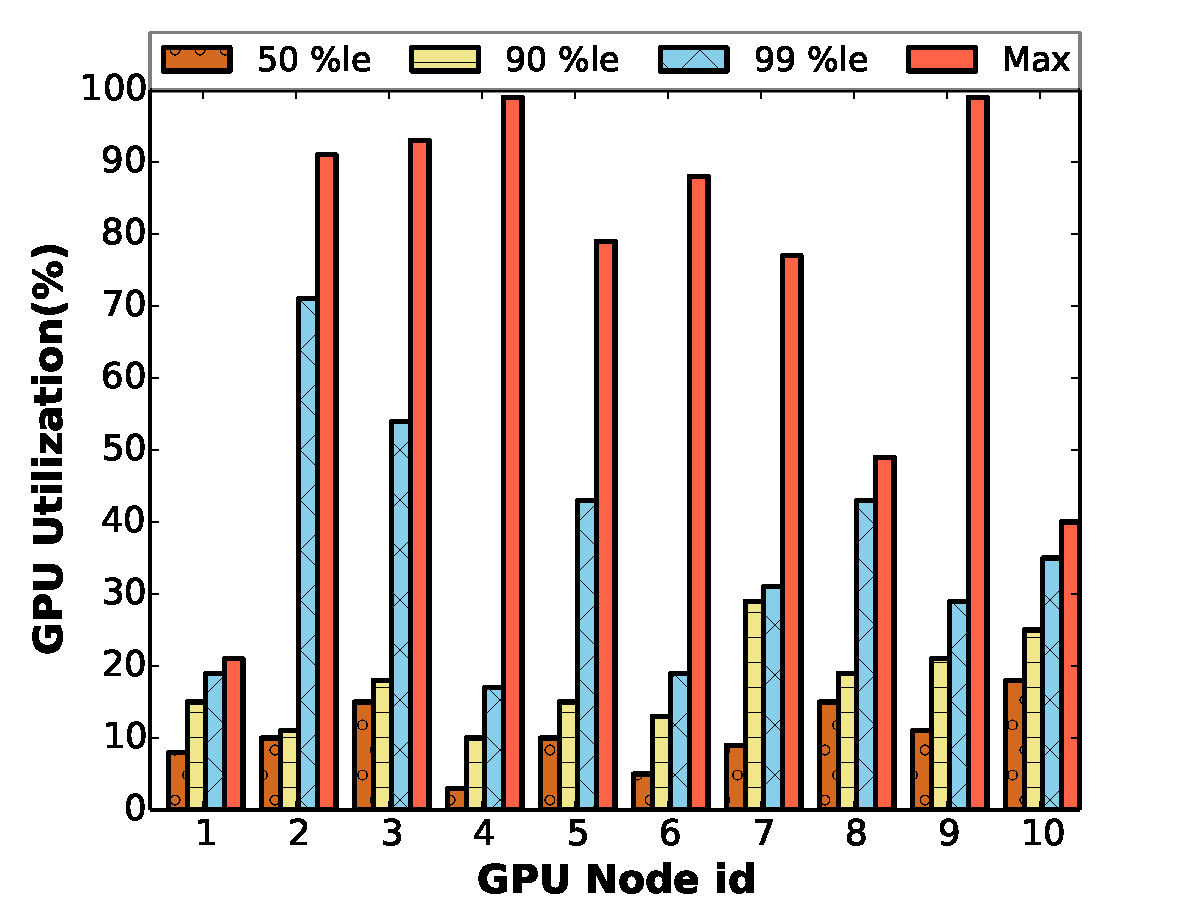
\includegraphics[width=1.1\linewidth]{results/app3-low.pdf}
  \caption{Application-Mix-3}
  \label{fig:app3}
\end{subfigure}
\vspace{-7mm}
\caption{50/90/99$^{th}$ percentile \& maximum GPU utilization for different application mixes scheduled using uniform scheduler.}
\label{fig:uniform}
\end{figure*}

\begin{figure}[tbp!]
\begin{subfigure}[b]{0.15\textwidth}
  \centering
  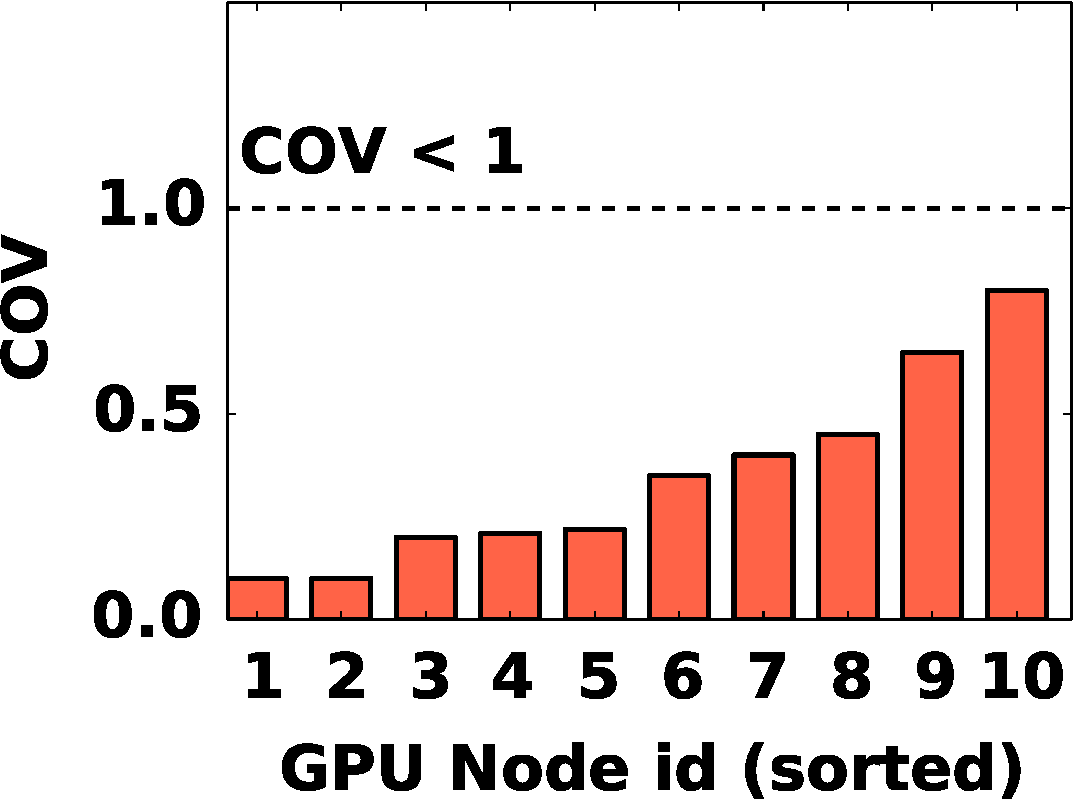
\includegraphics[width=.99\linewidth]{figs/app1-cov.pdf}
  \caption{App-Mix-1}
  \label{fig:app1-cov}
\end{subfigure}
\begin{subfigure}[b]{.15\textwidth}
  \centering
  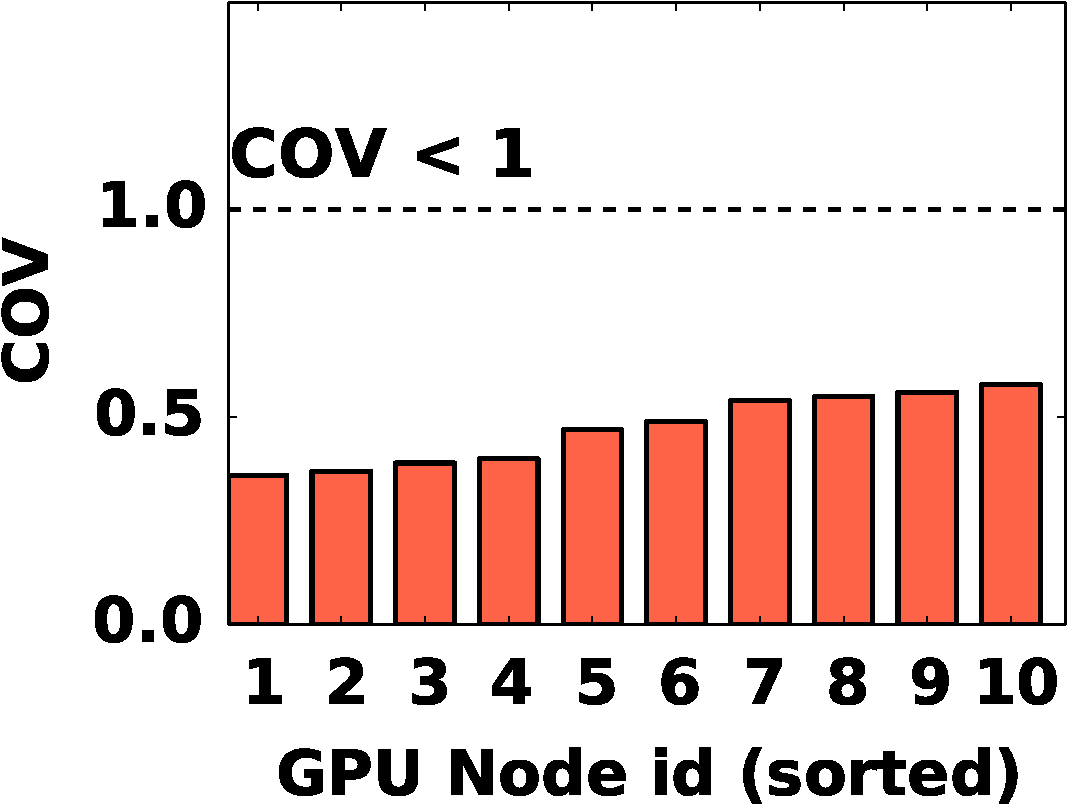
\includegraphics[width=.99\linewidth]{figs/app2-cov.pdf}
  \caption{App-Mix-2}
  \label{fig:app2-cov}
\end{subfigure}
\begin{subfigure}[b]{.15\textwidth}
  \centering
  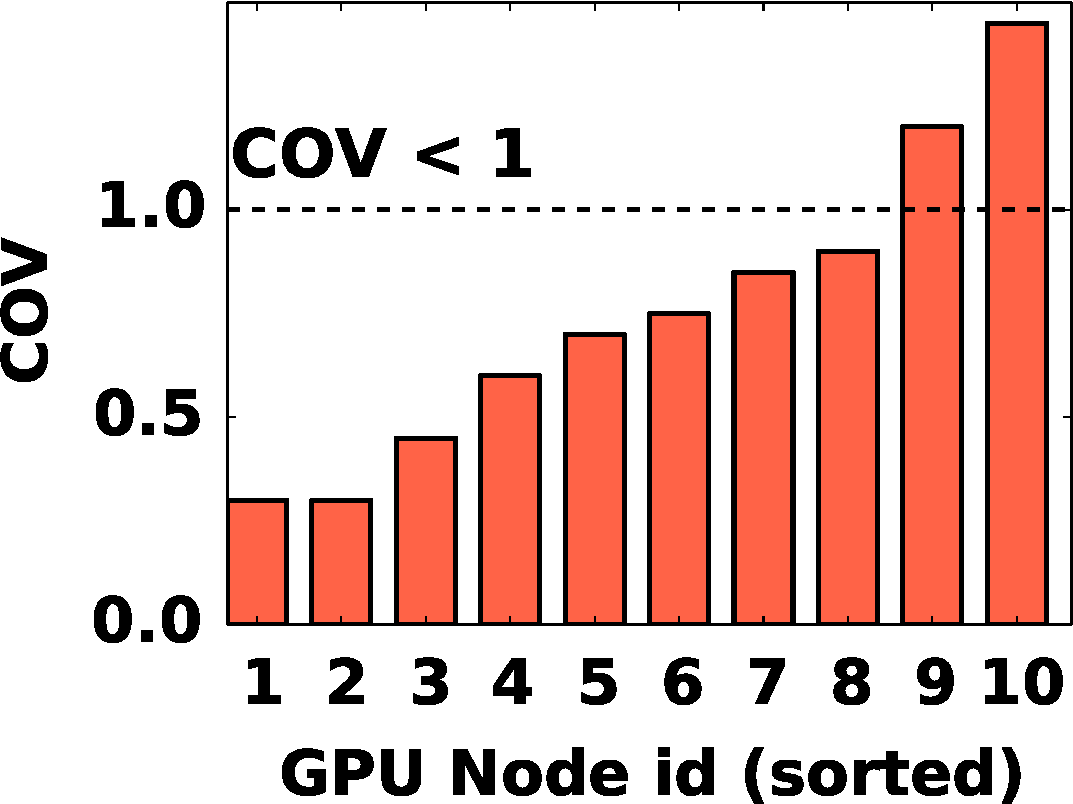
\includegraphics[width=.99\linewidth]{figs/app3-cov.pdf}
  \caption{App-Mix-3}
  \label{fig:app3-cov}
\end{subfigure}
\vspace{-2mm}
\caption{Coefficient of Variance across three Application-Mix.}
\label{fig:cov}
\end{figure}
\vspace{-2mm}


\subsection{Application-mix Analysis}
To schedule these workloads onto the GPU nodes, We use the \textit{Kubernetes} default scheduler, which uses the uniform scheduler to schedule containers and queries in FCFS basis. This scheduling policy is simple and scalable. It works well when the capacity of the resource is in abundance like CPUs. By default, GPU sharing is disabled as it complicates the scheduler-level performance/QoS guarantees and to ensure fairness across different co-scheduled applications. We schedule the app-mix through the uniform scheduler and plot the 50, 90, 99$^{th}$ percentile GPU utilization along with maximum utilization of individual GPUs as seen in Figure~\ref{fig:uniform}. For app-mix1 (in Figure \ref{fig:app1}) the 50$^{th}$ percentile utilization is much closer to 90$^{th}$/99$^{th}$ percentile utilization when compared to app-mix-3 (in Figure \ref{fig:app3}). This implies that the application load of app-mix-1 is \textit{higher} than app-mix-3, as we classified in Table \ref{tbl:appmix}. On the other hand, app-mix-2 in Figure \ref{fig:app2} has the 50\textsuperscript{th} to 99\textsuperscript{th} percentile evenly spaced. This also correlates to the classification we make for app-mix-2 in Table \ref{tbl:appmix} (indicates \textit{medium} load). %In these cases, both the 90,99$^{th}$\%le values are very close to the maximum GPU utilization. It also is critical to analyze the skew of the app-mix-3's utilization distribution in Fig~\ref{fig:app3}. It can be observed that the 50 and 90$^{th}$\%le GPU utilization is significantly less than 99$^{th}$\%le and the maximum utilization in most of the cases. This because the nature of the applications scheduled in this mix exhibit high variation in its resource demands though the aggregate utilization is low. This nature of the application also aligns with our observations made from Figure~\ref{fig:rodinia-peaks}. It is evident from these observations that the application usually overstates its resource requirements.

It is evident that, the applications have varying resource needs throughout their lifetime. Also, the applications always overstate their resource requirements by considering only for the peaks in the utilization  (also seen in Figure \ref{fig:rodinia-peaks}). This leads to under-utilization and queuing delays which directly results in poor energy efficiency and significant QoS violations, respectively. An efficient resource scheduler should leverage this dynamic workload behavior and incorporate policies that can guarantee the QoS while keeping the utilization high and improving energy efficiency. 

% If we could size an application based on 90-percentile CPU utilization instead of maximum CPU utilization, it could lead to significant savings. We also look at the other GPU utilization in Figure~\ref{fig:app2} and find that the observations to hold good even in case of average utilization.

\subsection{Utilization Variance Across GPU Nodes}
We also look into the variability in GPU utilization across the three different application mixes through the coefficient of variation(COV). COV is measured by the ratio of standard deviation $\sigma$ and mean $\mu$. This metric is a good indicator of the variations in the performance demands of the respective application mix. An application-mix with higher COV values are considered high in variance and harder to guarantee the performance when scheduled to the nodes. Consequently, those with COV$\leq$1 exhibit predictable workload consumption. It also makes it easier to guarantee the performance of an application to be scheduled to those nodes. Further, co-locating a heavy-tailed distribution (COV$\geq$1) to a positively correlated distribution with decaying tail (COV=1) would lead to application interference(noisy-neighbor) and severe capacity violations.
%\jash{relate noisy with spearman}

We sort the COV for all GPU nodes within an application mix and show it in Figure~\ref{fig:cov}. We observe that the COV is less than 1 for both app-mix-1 and app-mix-2. Therefore, it is easier to predict and guarantee while scheduling in those scenarios. In case of app-mix-3, the COV is greater than 1, and these applications have very low resource consumption. It is important for a GPU scheduler to take this into account while scheduling an application. If the scheduler is agnostic to the real-time utilization of the GPU, it will lead to co-location that results in heavy-tail distribution (e.g, time quantum 410-690 in Figure \ref{fig:rodinia-peaks}) resulting in pod failure. Hence it is important for a GPU orchestrator to provision for an application considering the real-time utilization metrics.
% hiding container launch latency while doing proactive admission control
% heterogeneous GPU allocation for bandwidth bound kernels to peak efficiency 
% inference workloads
% GPU performance prediction using ARIMA 
% Propose energy-aware scheduling schemes for tasks with energy constraints


% Node-level sharing related work comparison and problems
% Eg., non-preemptable accelerator issues demand smarter scheduling at first

% If shared what is the problem?
% Multi-container packing issues like memory crashing
% why? Underutilization of active memory across containers in GPU using 3 workloads
% Key factors: Memory,PCIe bandwidth,Queuing delay
% Predicting the container memory and saving container crashes

% Monitoring container usage on GPUs
% Proactive admission control and orchestration
% under-utilization, non pre-emptibility of GPUs, QoS guarentee, 
% Microservices and container framework

% Memory underutilization
% Energy
% exsiting TF library over commitment


%%%%%%%%%%%%%%%%
%\vspace{-0.15in}

%%------------------------------------------------------------------------------------------------------------------
\section{GPU-AWARE SCHEDULING} 
\label{sec:scheme}
In this section, we discuss different scheduling schemes that leverage \textit{Knots} framework to perform GPU-aware scheduling. These schemes are designed to leverage the design point findings from the Section \ref{sec:modeling}. 


% \begin{itemize}[wide, nosep, labelindent = 0pt, topsep = 0.3ex]

% \item \textbf{GPU Sharing Disabled - } This scheme is built to leverage our \textit{Knots} orchestration layer which could take advantage of the real-time GPU utilization metrics. Since Knots can query the utilization aggregator, this guarantees the end-to-end QoS of the service queries.

% \item \textbf{GPU Sharing Enabled - } expanded as Auto-Regressive Integrated Moving Average based scheduler, which uses moving window based regression to forecast the GPU resource usage to predict the device utilization.
% \end{itemize}

% \vspace{0.2in}
\subsection{Uniform container scheduling}
\textit{Kubernetes} uses uniform scheduling of containers (pods) which optimizes the use of one resource ( core utilization) through uniform bin packing and treats other resources (e.g., memory, I/O) as constraints. Note that, a GPU is considered as a scheduling constraint, while ignoring the actual device utilization. It uses static placement, which does not ensure load balancing. This scheme scales well with the increase in resources and always comes up with a possible bin packing mechanism for all applications. But, it does not allow sharing of resources across applications. The three application mixes shown in Table~\ref{tbl:appmix} are scheduled using uniform scheduler. We use this scheme as our baseline.

Figure~\ref{fig:uniform} shows the utilization of each of the ten GPU nodes. Uniform scheduler is actually better in cases where the utilization is already high (for instance application-mix-1 from Figure~\ref{fig:app1}). \textit{Kubernetes} depends on application frameworks (for instance Spark \cite{spark}, Tensorflow) to manage its resources internally. From \textit{Design point 5}, we know that it is ideal to expose the application framework's parameters to the cluster scheduler to avoid any internal resource fragmentation as seen in Figure~\ref{fig:tf-frag} (TF - the top line in red consuming 98\% of the memory). Instead, these idle resources could be allocated to the pending pods by sharing the resource. We configured the Tensorflow (TF)'s GPU configuration parameters in such a way that the framework does not subscribe to the entire GPU memory by allowing memory growth for each task. This enables us to pack the GPUs with other pending pods leading to the second scheme.

\vspace{-0.1in}
\subsection{Resource agnostic sharing}
We enable scheduling of multiple containers (pods) on a single GPU by modifying the Nvidia's k8s-device-plugin~\cite{k8s} for Kubernetes. We used first fit decreasing order bin-packing algorithm which greatly improves the average GPU utilization and job turnaround times hiding the container start-up latencies. This trend is consistent with our previous observations that led to \textbf{Design point 1}. GPU-sharing satisfies the \textbf{Design points 1 \& 3} which is maximizing the utilization by enabling  resource sharing and keeping the utilization high for power proportionality respectively. However, it fails to consider the actual GPU utilization, while scheduling and this leads to severe QoS and capacity violations (discussed in \textbf{Design Point 2}). When GPU sharing is enabled, it is important that the cluster-wide resource scheduler should take the application characteristics and the resource utilization to safely schedule the containers (pods). At production scale it becomes an overhead to guarantee the pod safety. Hence, \textit{Kubernetes} does not explore sharing as an option, which led to our next scheme.
\vspace{-0.1in}
\subsection{Correlation Based Provisioning}
Following the observations made from Alibaba cluster trace, in order to make effective scheduling decisions, the correlation between the utilization metrics must be used for proactive application placement, especially when GPU sharing is enabled. Since \textit{Knots} leverages the utilization aggregator to collect the real-time utilization statistics from the GPU, the scheduler can leverage this information to predict whether the pods can be co-located. For example, two pods positively correlating for using the GPU memory should be scheduled to different GPU nodes as the pods have a high probability of memory capacity violations when co-located. Note that, such capacity violations can lead to container crashing and relaunching. Although the relaunch latency is typically in the order of few seconds, the tasks when relaunched cannot be prioritized over tasks of other pods that are already ahead on the queue. In this case, this particular heavy tailed task affects the overall job completion time. Therefore, the correlation based prediction (CBP) scheduler avoids co-locating two positively correlating pods for any metric such as memory, SM load and bandwidth.

%Therefore, if we size applications based on dominant resource metric~\citep{Ghodsi:2011:DRF:1972457.1972490} agnostic of their correlation metric, there is a high chance of QoS violation due to heavy-tailed tasks.

As we observed in Figure~\ref{fig:rodinia-peaks}, all the representative GPU batch workloads have significantly low peak resource usage for most of their execution. For example, SM utilization has a 90x difference between its median and peak. Similarly, bandwidth utilization differs by 400x between the median and peak. The application uses the whole allocated capacity only for 6\% of the total execution time, but it is always provisioned for the peak utilization . This leads to resource fragmentation and underutilization. Hence, this property can be exploited by pod resizing. For example, if two uncorrelated applications are containerized as pods and placed individually, they have an X\% probability of failure. Whereas if they are co-located, they have a probability of failing together, which is $1-( {1 - X})^2$. Hence, provisioning based on an average usage and packing uncorrelated applications together can lead to potential savings over res-ag scheduling. We call this scheme correlation based provisioning (CBP) which resizes the uncorrelated pods for efficient packing on GPUs.

CBP scheduler takes \textit{\textbf{O$(N^2d)$}} to find the optimal placement where N is the number of pending pods and \textit{\textbf{d}} being the time-series window size which is a crucial configuration parameter that determines the scheduling accuracy. CBP scheduler bin packs the uncorrelated applications together by resizing their respective pods for a common case (90$^{th}$ percentile consumption) than for the maximum case. We conservatively provision for 90$^{th}$ percentile, since aggressive provisioning (Viz. 50$^{th}$, 60$^{th}$, etc.) affects docker performance and constant resizing makes the GPU docker environment unstable. CBP is based on our observations that the probability of all co-located pods reaching their peak consumption at the same time is very low. Thus, CBP is aware of both utilization and the pod's correlation metrics. However, due to conservative provisioning the GPUs are still under-utilized. This could be also due to the interarrival pattern of pods, since there are not enough negatively correlating pods to co-locate which results in a skewed schedule order. This indirectly restricts the potential number of GPU nodes to schedule the pods and results in increased queue waiting times for the pending pods which are positively correlating. The average pod waiting time worsens especially in case of heavily loaded application-mix. Pod affinities would further restrict scheduling options for correlating pods. This leads us to our next scheme that attempts to co-locate two positively correlated pods in the same node by predicting the peak resource demand phases of the scheduled pods.


\subsection{Peak Prediction Scheduler}
Peak Prediction scheduler is built on top of CBP to further exploit the temporal nature of peak resource consumption within an application. This allows PP to schedule two positively correlating pods to the same GPU as they may not contend for the resource at the same time. This is due to the fact that a single application goes through several phase changes during its course of execution. For instance, a DNN instance query first loads the inference weights from the host which results in peak input bandwidth consumption, this is followed by the next phase of the application that is the compute/memory intensive phase. This trend is also very evident in batch workloads as seen in Figure~\ref{fig:rodinia-peaks}. Thus, the peak bandwidth consumption of an application is an early indicator of subsequent compute and memory peaks. Likewise, within an application, the consecutive peak resource demand trends can be predicted using the auto-correlation function given in Equation~\ref{eqn:auto}, r$_{k}$ being the auto-correlation value where Y$_{i}$ is the utilization measurement at a given time, $\bar{Y}$ is the moving average of Y, and n is the total number of events record at a time window T. 

\begin{equation} 
r_{k} = \frac{\Sigma{_{i=1}^{n-k}} (Y_i - \bar{Y})(Y_{i+k} - \bar{Y})} {\Sigma{_{i=1}^{n}}{(Y_i - \bar{Y})}^2}
\label{eqn:auto}
\end{equation}

The utilization metric can be further forecasted to anticipate the future GPU utilization using non-seasonal Auto-Regressive Integrated Moving Average(ARIMA). The interval between two consecutive peak resource consumption of a particular resource could be determined by the auto-correlation factor. If the auto-correlation value of a series (i.e., memory utilization) is zero or negative then it shows that (i) the input time-series data is limited or (ii) the trend is not strong enough to predict a positive correlation. In case of correlation value being greater than 0, we use first-order ARIMA to forecast the utilization of the GPU for the next one second as given in Equation~\ref{eqn:arima} below which is a moving window based linear regression where $\hat{Y}$$_{pred}$ is a predicted utilization value from previous utilization timeseries $Y_{t-1}$, where $\phi$ is the slope of the line and $\mu$ is the intercept.
    \begin{equation} 
    \hat{Y}_{pred} = \mu + \phi_{1} Y_{t-1}
    \label{eqn:arima}
    \end{equation}

 


%%%%%%%%%%%%%%%%%%%%%%%%%%%%%%%%%%%%%%%%%%%%%%%%%%%%%%%%%%%%%%%
\begin{algorithm}
\caption{ CBP + Peak Prediction Scheduler}
\begin{algorithmic}[]
%\footnotesize
%\Procedure{Recursion}{$a$}
%\State $a\gets\textsc{Recursion}(a)$ \Comment{Call Recursion again}
%\EndProcedure
\NoDoFor{\textit{gpu\_node in $\forall          all\_gpu\_nodes$}}
\If{isActive(\textit{QUERY(gpu\_node)})}

\State$\textit{All\_Active\_GPUs.append}(\textit{gpu\_node})$
\EndIf
\EndFor
\State$\textit{Node\_List} \gets \textit{Sort\_by\_Free\_Memory(\textit{All\_Active\_GPUs})}$
\State$\textit{Pending\_Apps} \gets \textit{Sort\_Apps\_by\_Memory\_Size(Apps)}$
\State$\textit{Resized\_apps} \gets \textit{Docker\_Resize(Node\_List,Pend\_Apps)}$
\State$\textit{Selected\_Node} \gets \textit{Head(Node\_list)}$
\NoDoFor{\textit{App in Pend\_Apps}}
\State$\textit{Schedule(app,Selected\_Node)}$
\EndFor
\Procedure{Query(\textit{GPU\_node})}{}

\State$\textit{node\_stats\_mem} \gets \textit{query\_db(gpu\_node.memory)}$
\State$\textit{node\_stats\_sm} \gets\textit{query\_db(gpu\_node.sm)}$
\State$\textit{node\_stats\_tx} \gets\textit{query\_db(gpu\_node.tx\_band)}$
\State$\textit{node\_stats\_rx} \gets\textit{query\_db(gpu\_node.rx\_band)}$
\State$\textit{node\_stats} \gets \textit{node\_stats\_mem} + \textit{node\_stats\_sm} + \textit{node\_stats\_bw}$
\State$\Return \textit{   node\_stats}$
\EndProcedure

\Procedure{Schedule(\textit{App, Selected\_Node})}{}
\If{\textit{Can\_Co-locate}(\textit{Covariance,App,Selected\_Node})}
\State$\textit{Ship\_Container(App,Selected\_Node)}$
\Else{}\\

\If{\textit{AutoCorrelation(node$.$memory)}} \Comment{\textbf{\textit{Eqn \ref{eqn:auto}}} }
\State$ \textit{pred\_free\_mem} \gets \textit{ARIMA(node$.$mem)}$
\If{\textit{pred\_mem $\ge$ App$.$memory }}
\State$\textit{Schedule(app)}$
\Else{}
\State$\textit{Schedule}(\textit{App,Head$\,\to\,$Next(Node\_list})$
\EndIf
\EndIf
\EndIf
\EndProcedure
% \Procedure{Compute\_CRV(Constraint)}{}
%  \State
% \EndProcedure
\end{algorithmic}
\label{algo}
\end{algorithm}
%%%%%%%%%%%%%%%%%%%%%%%%%%%%%%%%%%%%%%%%%%%%



Note that, the correlation between consecutive peak resource consumption is a better indicator than the correlation across complete runtime of the application. Also, forecasting the GPU utilization enables the system scheduler to predict the performance better and guarantee the QoS of the application which would be scheduled to that particular GPU node. The peak prediction scheme identifies the set of pods that attains peak consumption of a resource at the same time and schedules them to different GPU nodes.

Algorithm~\ref{algo} captures the workflow of the scheduler, where for all the active GPU nodes in the datacenter, the utilization for the past five seconds is queried from the respective influxdb databases. This timeseries window could be adjusted for prediction accuracy. The utilization aggregator in the headnode sorts the nodes by free memory available for the most recent timestamp. The schedule order of pending pods is sorted based first fit decreasing order of pod's requested memory and resized for 90$^{th}$ percentile memory consumption. The \texttt{Select\_Node} function further analyzes the correlation in case of CBP and schedules to the \texttt{Selected\_Node} in case of the correlation value is less than 0.5. In case of PP, the auto-correlation function is used on the utilization time-series data for a particular metric(memory\_used) of the selected node to look for a trend which predicts a possibility of an impending peak resource consumption to occur through ARIMA, in that case schedule to the next available node in the list by repeating the same admission checks. Once the node is selected, the pod is shipped to the node using \textit{Kubernetes}'s python-based client API calls.


% However, two applications with correlated peaks may still be co-located. 
% 3) Co-located applications that do peak together can use a common buffer for their peaks, and each has a reservation equal to an off-peak value. Using these ideas first to identify clusters of applications with correlated peaks,  one may observe that the number of such clusters may become very large if we use the original time series with the complete range of values. Hence, Peak uses a novel two-level envelop of the original time-series of each application for clustering. The envelope has a single value to represent all CPU utilization for the body of the distribution and another value for all points in the tail of the distribution. On each active server, it then reserves space for each cluster in proportion to the size (lower level of the envelope) of the applications in that cluster and keeps a buffer space equal to the maximum peak across all clusters. Each application cluster narrows down a set of applications for its reservation.




%%------------------------------------------------------------------------------------------------------------------
\section{EVALUATION METHODOLOGY}
\label{sec:methodology}

\begin{table}[t]
\begin{minipage}{.45\linewidth}
\begin{center}
\resizebox{\textwidth}{!}{
 \begin{tabular}{||p{1.3cm}| p{2cm}|} 
 \hline
  \textbf{Hardware}  & \textbf{Configuration}\\
 \hline
 \textit{CPU}  & Xeon E5-2670 \\
 \hline
 \textit{Cores} & 12x2(threads) \\  
  \hline
  \textit{Clock} & 2.3 Ghz \\
  \hline
  \textit{DRAM} & 192 GB \\
  \hline
  \textit{GPU} &  P100(16GB) \\
  \hline
%   \textit{GPU2} & K80(12GB)x2 \\
%   \hline 

  \end{tabular}}
\end{center}

\caption{Hardware config}
\label{tbl:hw-config}

\end{minipage}%
 \hspace{2mm}
\begin{minipage}{.45\linewidth}
\begin{center}

 \resizebox{\textwidth}{!}{%
 \begin{tabular}{|p{1.8cm}| p{2cm} ||} 
 \hline
   \textbf{Software} & \textbf{Version} \\
   \hline
   \textit{Kubernetes} & 1.9.3 \\ 
%    \hline
%    \textit{Docker} &  2.9 \\ 
   \hline
   \textit{NvidiaDocker} &  2.0 \\
   \hline
   \textit{pyNVML} & 7.352.0 \\ 
   \hline
   \textit{InFluxDB} & 1.4.2  \\ 
   \hline
   \textit{CUDA} & 8.0.61 \\ 
   \hline
   \textit{Tensorflow} &  1.8 \\
  \hline
\end{tabular}}
\end{center}

\caption{Software config}
\label{tbl:sw-config}
\end{minipage}%
\end{table}
% \vspace{-0.1in}
\subsection{Experimental setup}
%\begin{itemize}
%\item{\textbf{Hardware:}}
\subsubsection{Hardware}

We use Dell PowerEdge R730 eleven node cluster where ten worker nodes have P100 GPUs with Intel Xeon CPU host along with a CPU-only head-node. The details of the single node hardware configuration are listed in the Table~\ref{tbl:hw-config}. We use \textit{Kubernetes} as the resource orchestrator and its default uniform scheduler as our baseline.
\begin{itemize}[wide, nosep, labelindent = 0pt, topsep = 0.3ex]
\item{\textbf{Worker node -}} At every GPU worker node, there is a node-level resource monitor that uses python based API library, pyNVML~\cite{pynvml} to query the GPU for every heartbeat interval. The query returns all the five utilization metrics namely, SM, memory, power, transfer and receive bandwidth. These metrics are logged as time-series data into the Influxdb database in their respective nodes.
\item{\textbf{Head node -}} The configuration is similar to that in Table~\ref{tbl:hw-config}, with an exception that it does not have a GPU. Next, the utilization aggregator on the head node queries the real-time GPU utilization from the Influxdb. The frequency of querying interval is set to 1ms ( justified in Section \ref{sec:picking}). The frequency of data logging (heartbeat) can be varied at the discretion of the utilization aggregator as seen in Figure~\ref{fig:kubeknots}.
\end{itemize}
%\item{\textbf{Container setup:}}

\begin{figure*}[!tbp]
\begin{subfigure}[b]{0.33\textwidth}
  \centering
  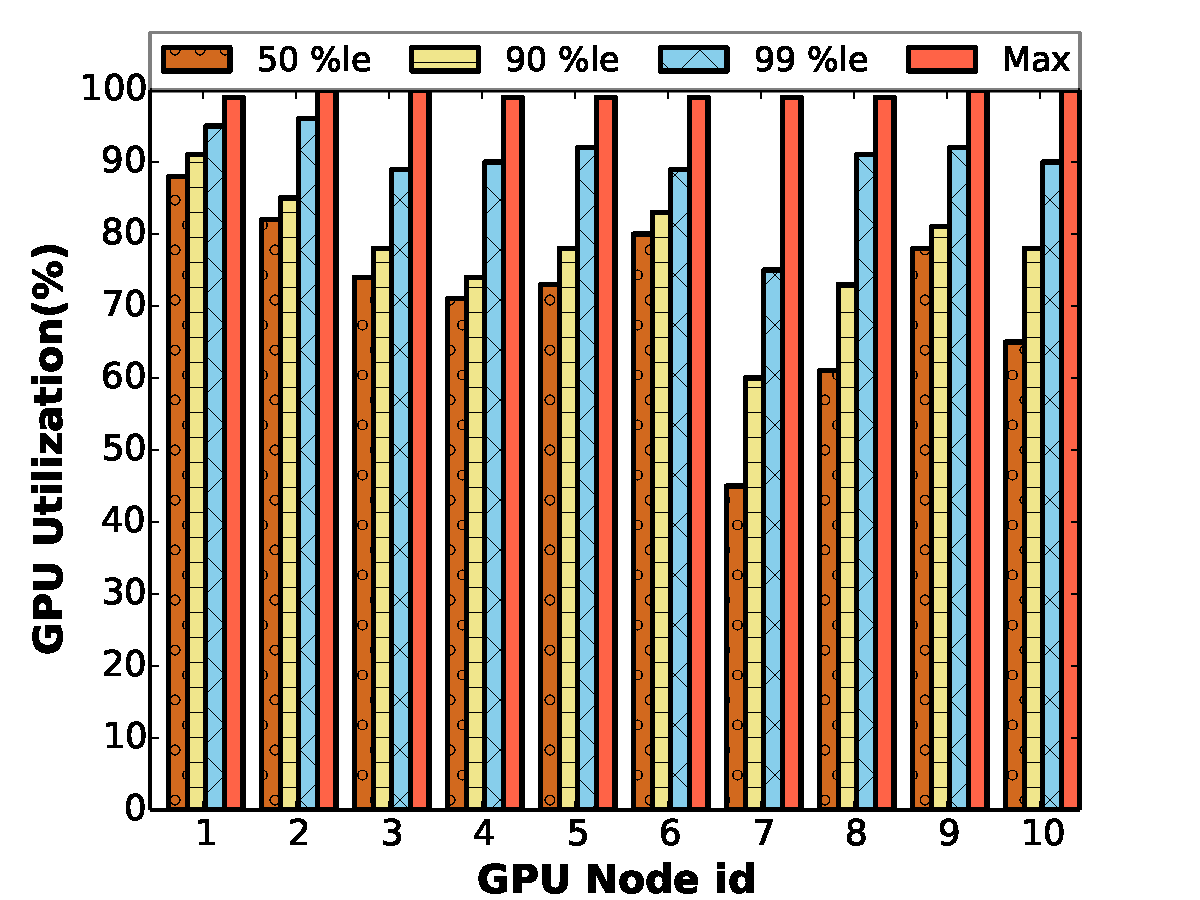
\includegraphics[width=1.1\linewidth]{results/app1-peak.pdf}
  \caption{Application-Mix-1}
  \label{fig:app1-pcp}
\end{subfigure}
\begin{subfigure}[b]{.33\textwidth}
  \centering
  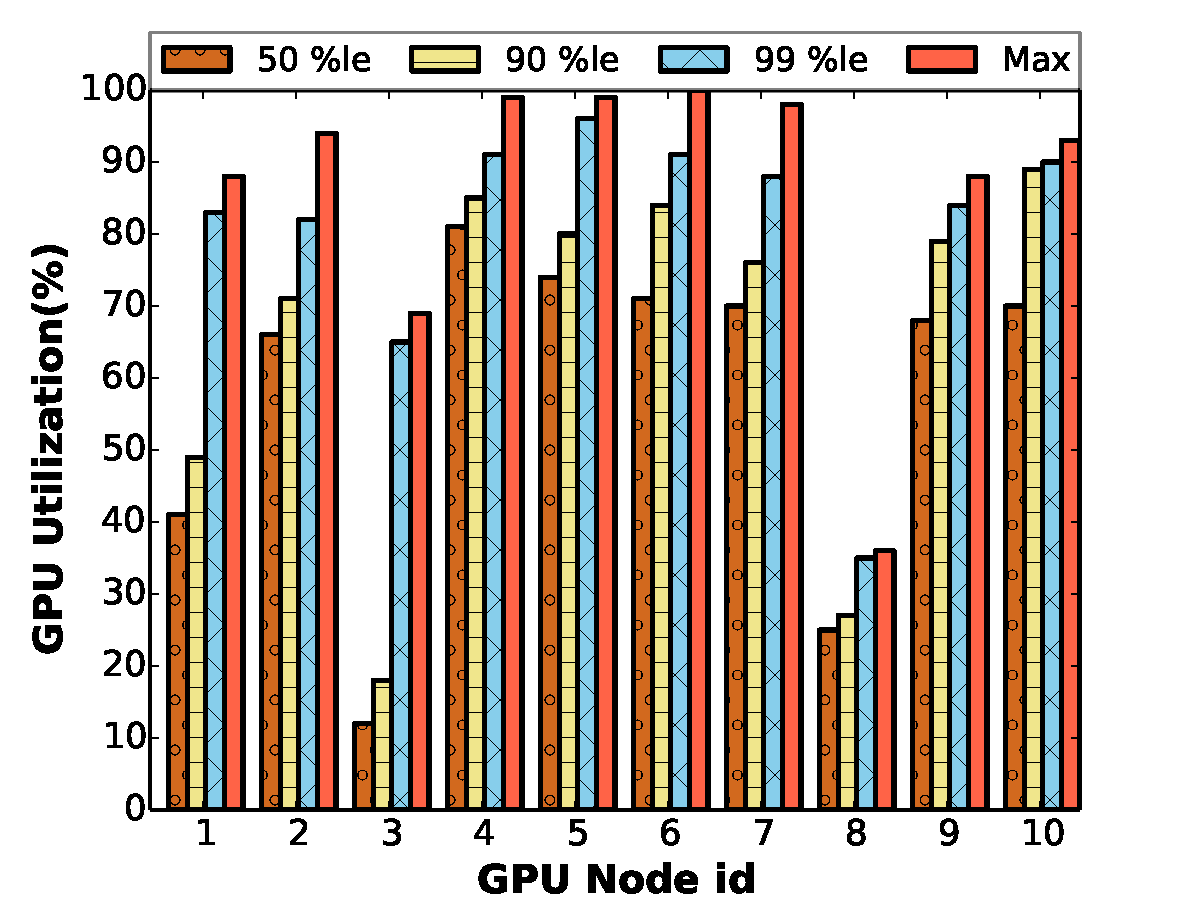
\includegraphics[width=1.1\linewidth]{results/app2-peak.pdf}
  \caption{Application-Mix-2}
  \label{fig:app2-pcp}
\end{subfigure}
\begin{subfigure}[b]{.33\textwidth}
  \centering
  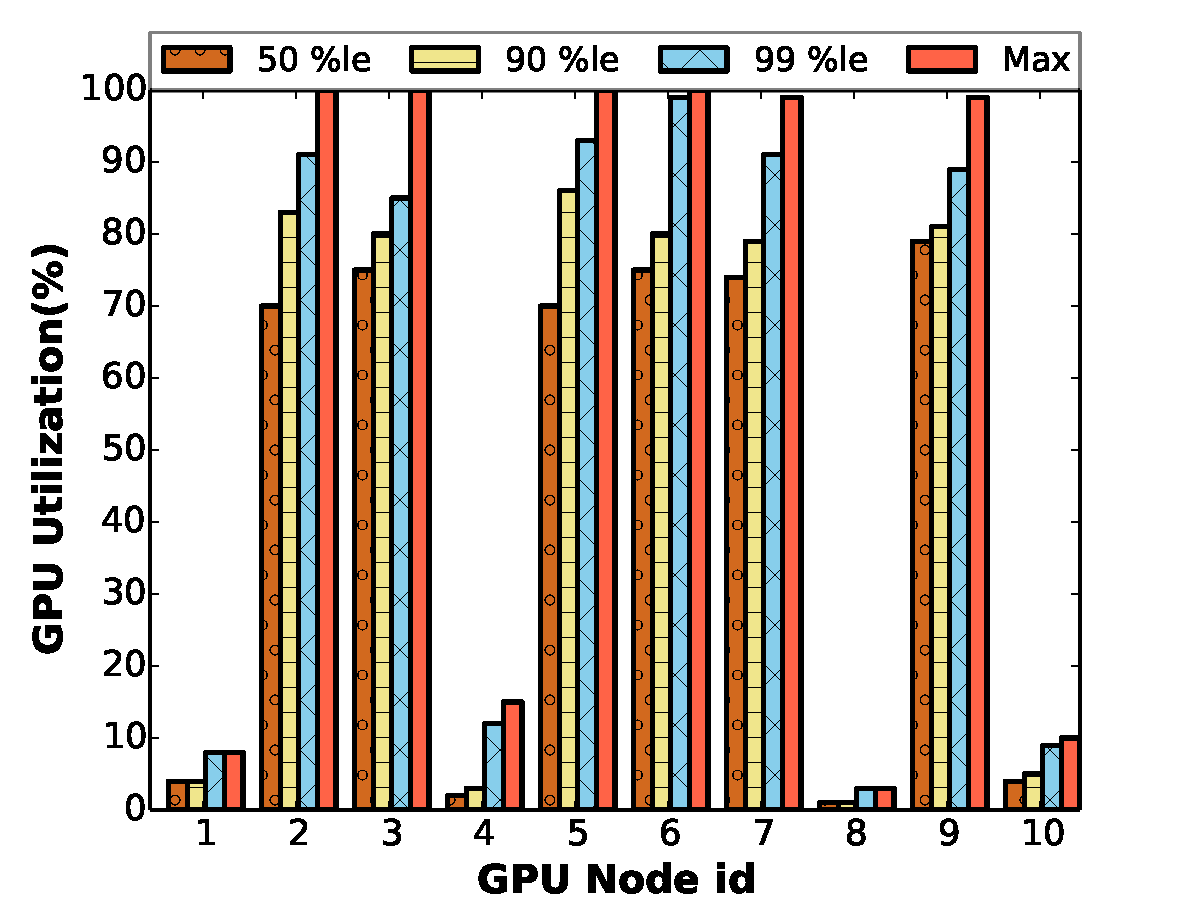
\includegraphics[width=1.1\linewidth]{results/app3-peak.pdf}
  \caption{Application-Mix-3}
  \label{fig:app3-pcp}
\end{subfigure}
\vspace{-6mm}
\caption{50/90/99$^{th}$ percentile \& maximum utilization of GPUs for App-Mixes scheduled using Peak Prediction Scheme.}
\label{fig:pcp}
\end{figure*}

\begin{figure}[tbp!]
\begin{subfigure}[b]{.15\textwidth}
  \centering
  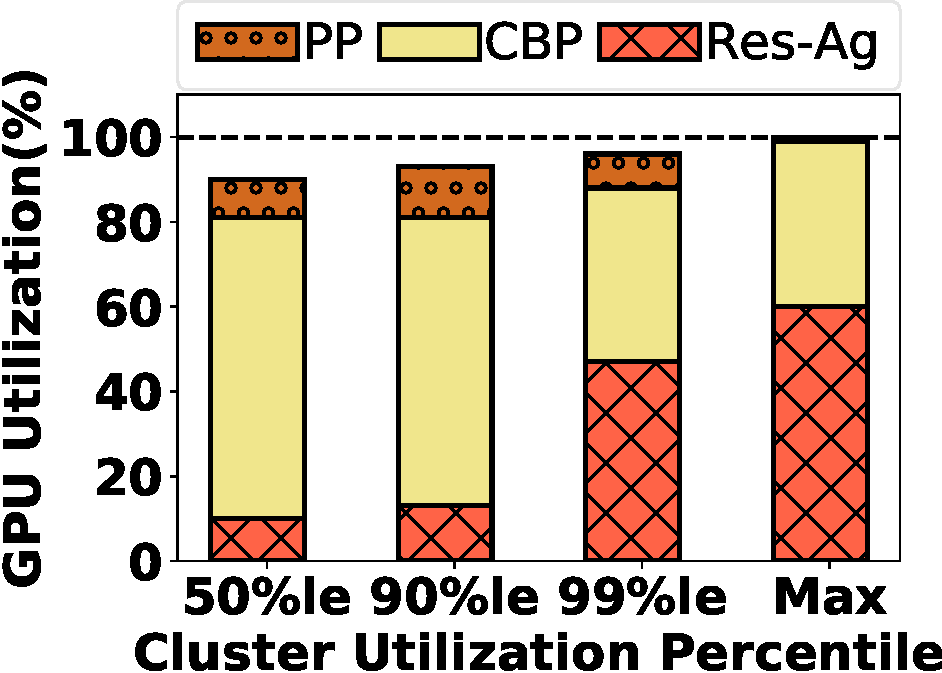
\includegraphics[width=.99\linewidth,height=2cm]{results/app1-avg.pdf}
  \caption{App-Mix-1}
  \label{fig:util1}
\end{subfigure}
\begin{subfigure}[b]{.15\textwidth}
  \centering
  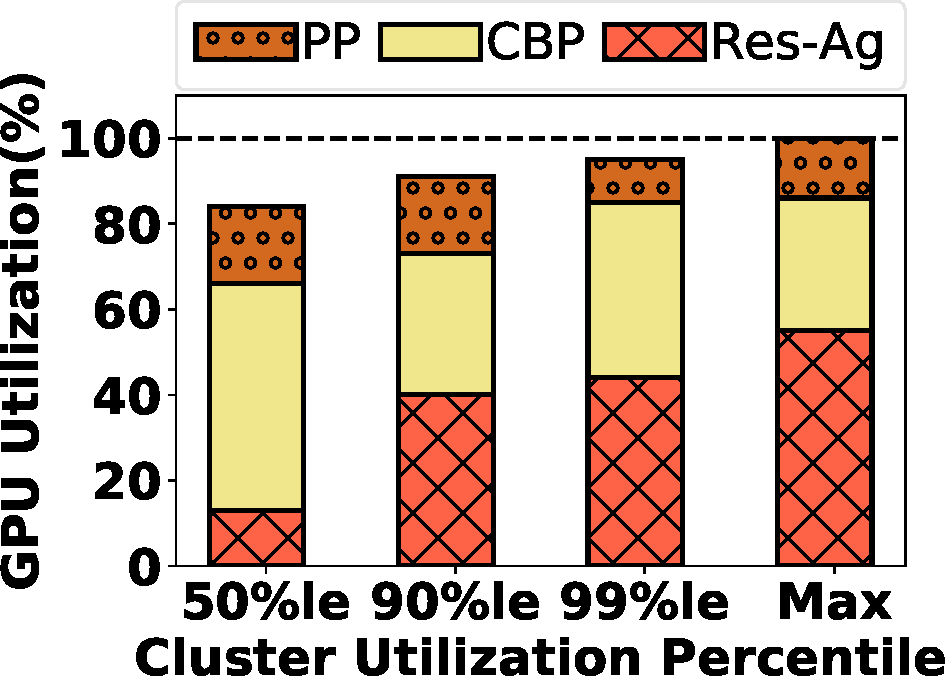
\includegraphics[width=.99\linewidth,height=2cm]{results/app2-avg.pdf}
  \caption{App-Mix-2}
  \label{fig:util2}
\end{subfigure}
\begin{subfigure}[b]{.15\textwidth}
  \centering
  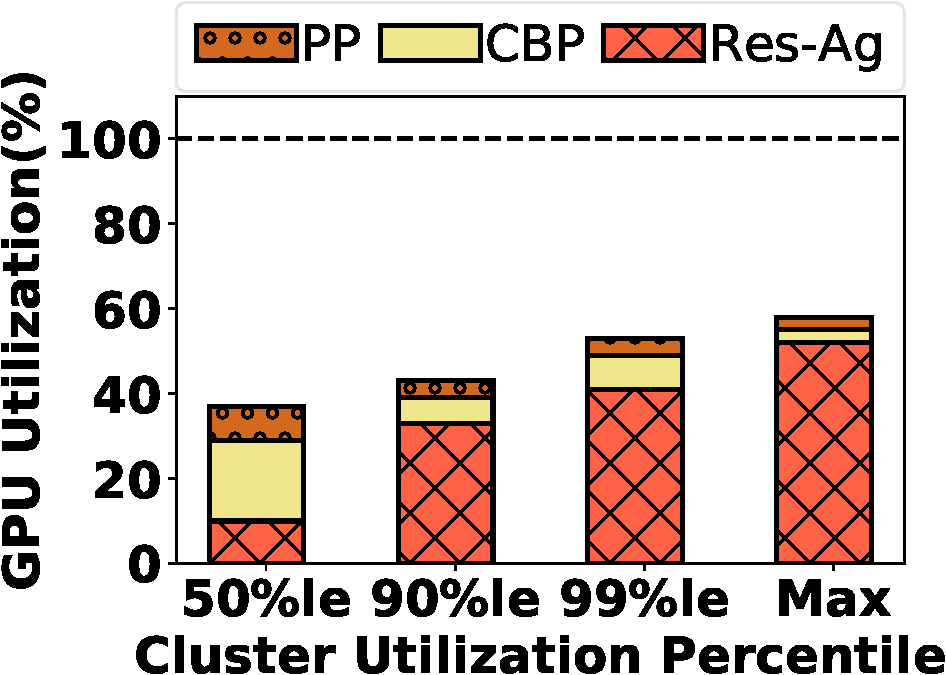
\includegraphics[width=.99\linewidth,height=2cm]{results/app3-avg.pdf}
  \caption{App-Mix-3}
  \label{fig:util3}
\end{subfigure}
\vspace{-3mm}
\caption{Cluster-wide GPU utilization improvements.}
\label{fig:util}
\vspace{-2mm}
\end{figure}

\subsubsection{Container Configuration}

Both the batch and user-facing applications are containerized as pods in \textit{Kubernetes}, and their image is made available in all the GPU nodes beforehand, to avoid any startup latencies. The software configuration is given in Table~\ref{tbl:sw-config} Since these containers are multi-GB and pre-packed with the datasets along with the workloads, the start-up latency depends entirely on the network bandwidth to download the container from a docker-hub or launch from the head-node. To avoid any unprecedented network delays while shipping these containers, we made sure all the nodes had the docker image of the respective workloads in advance. This way, a scheduler can potentially launch the application in any node for the same shipping cost (Typically, the image will be downloaded for the first time (cold start) and then will continue to persist until the container is killed). For application resizing, we used NVIDIA-docker commands to resize the containers before launching the application mixes dynamically. 

Recall from Section \ref{sec:modeling} that, for batch applications we used Rodinia~\cite{che2009rodinia}, HPC and scientific workload suite. Similarly, for latency critical workloads, we used Djinn \& Tonic workload suite~\cite{hauswald2015djinn} which has several DNN inference queries using Tensorflow(TF) on GPUs through Keras libraries for execution. We configured TF's GPU configuration knobs to allow incremental memory growth for the DNN inference queries.  We capture the inter-arrival pattern of the Alibaba trace which is representative of the datacenter workload. We incorporate this inter-arrival pattern in our launch sequence of jobs. The  job sequence comprises of a bin of application-mixes (refer Figure \ref{fig:cov}). 
%\end{itemize}
%\subsubsection{Workload setup}
 




%\subsection{Headnode setup}
%The query interval can be tuned further to improve the accuracy of our peak prediction model at the cost of device overheads due to intrusive monitoring.



%%------------------------------------------------------------------------------------------------------------------
\section{RESULTS AND ANALYSIS} 
\label{sec:results}




In this section, we evaluate the different GPU-based scheduling schemes for four major criteria: (i) Cluster-wide utilization, (ii) QoS violations, (iii) Power, and (iv) Accuracy of prediction.


\subsection{Cluster-wide GPU Utilization}
Building upon the uniform scheduler which does GPU-agnostic scheduling (shown in Figure~\ref{fig:uniform}), we propose three scheduling schemes: (i) Res-Ag (ii) CBP and (iii) PP. In Figure~\ref{fig:pcp}, we plot the  utilization improvements of each of the ten GPU nodes for every app-mix using the PP scheduler. The PP scheduler improves the utilization in all the three app-mixes by an average of 62\%. Especially in app-mix 2 and app-mix 3, where the utilization is medium and low respectively, the PP scheme does an effective consolidation of workloads using a minimal number of GPUs as possible. As seen in Figure~\ref{fig:app3-pcp}, GPU nodes 1,4,8 and 10 are minimally used as the scheduler effectively consolidated all the low demand workloads to a minimum number of active GPUs as possible. This consolidation shows that, PP leverages the real-time utilization along with utilization forecasting before making any scheduling decisions. 

Figure~\ref{fig:util} plots the overall resource utilization improvements for all three application mixes for median and tail percentiles. It can be noted that our PP scheme consistently improved the overall GPU utilization in all low, medium and high application-mix cases. For example, PP in app-mix-1 improves by 80\% for both median and tail percentiles when compared with Res-Ag scheduler. The improvements are also consistent in the other two app mixes where the improvement over Res-Ag scheduler for median and peak percentiles are 60\% and  45\% respectively. These benefits reaffirm our prior observation that, it is better to predict the peak resource consumption of the workloads.

~\subsection{QoS of latency critical workloads}
~\label{sec:qos}
QoS violation threshold for latency-sensitive applications is typically set around 150 milliseconds \cite{Dean}. When end-to-end latency of such queries exceeds 150ms, they have to be relaunched. We show in Figure~\ref{fig:qos} that the baseline scheduler violated QoS by 18\% on average even though the applications are not co-located together. This is because of queuing delays, where the query is sent to a busy GPU node. The Res-Ag performs worse than the baseline and violates the threshold from 10\% (app-mix-3) to 53\% (app-mix-1) of the requests. On the contrary, CBP and PP have almost no violations in all three app-mix ($<$1\%). This is because these schemes were aware of real-time GPU utilization and provisioned the containers for 90 percentile utilization while guaranteeing the QoS via utilization forecasting. 
{Note that, we also co-locate the latency sensitive queries along with the batch jobs without affecting their QoS. PP achieves this by predicting the inter and intra-application correlation for utilization and, at the same time by leveraging Knots real-time data, it can forecast the future node utilization. This avoids QoS violations while keeping the utilization high.}

Since \textit{Knots} exposes the GPU utilization through Nvidia's resource monitoring APIs, the schedulers built on top of \textit{Kube-Knots} inherently take advantage of these metrics. Figure~\ref{fig:load} plots the pair-wise COV of GPU cluster loads. The lower diagonal values are omitted for the sake of clarity. It can be observed that the COV of loads across different GPU nodes ranges within 0 to 0.2 when compared to the COV in Figure~\ref{fig:app1-cov} which ranges from 0.1 to 0.7. Hence, PP performs load balancing in high-load scenarios such as app-mix-1 along with consolidation in low-loads such as app-mix-3.


%The GPU scheduler provides feedback to the workload balancer about how efficiently a pod is using the GPU, by computing GPU utilization, as the ratio of the total GPU time of an application to its total runtime. These decisions are refined over time as the system learns about the GPU characteristics of more pods from the feedback. 


~\subsection{Power efficiency}

All three schedulers namely Res-Ag, CBP, and PP consume less power than the uniform scheduler. Where, Res-Ag consumes the least power on an average (33\%) while PP scheme consumes the second least power (43\%). Note that, while Res-Ag optimizes for power it also violates QoS for almost 53\% of the requests as discussed in section \ref{sec:qos}. On the other hand, the PP scheduler only consumes 10\% more power than Res-Ag while guaranteeing minimal QoS violations. This is due to the fact that, although the PP scheduler attempts to pack only active GPUs but it ensures that two pods do not peak for resource consumption at the same time.

The CBP scheme consumes more power than both Res-Ag and PP schemes by 25\% and 15\% respectively, although being similar to PP scheme in terms of QoS violations. This emphasizes the importance of predicting the peak resource consumption of pods on top of the correlation metrics. We next understand the impact on of PP scheduler's accuracy by varying the frequency of the querying interval.

\begin{comment}

{As we discussed in Section \ref{sec:methodology}, high GPU utilization (especially at 90 and 99$^{th}$ percentile) causes better consolidation. As a consequence, we also observe an improvement in power consumption. For the three app-mixes, we aggregate only the GPU power consumed over the application run-time across different nodes by probing them every 1 millisecond. Then, we plot the average power consumed across all GPUs for all app-mixes when scheduled with the three different schedulers in Figure~\ref{fig:power}. For example, app-mix-1 consumes only 50\% of the power consumed when scheduled using PP scheduler over the baseline uniform scheduler and 25\% less power when compared to CBP scheduler. Although this trend holds in app-mix-2 and app-mix-3, res-ag scheme consumes less power than our proposed PP scheme in app-mix-2 by 30\%.}. 
{A striking observation to be made is that the resource utilization agnostic(Res-Ag) scheduler gives best power efficiency as it tries to bin pack the applications in round-robin without any QoS considerations at all. Thus Res-Ag improves the power efficiency by 50\% in app-mix 1 and 80\% in both app-mix2 and app-mix-3. Our second scheme, CBP is less power efficient than ResAg, but still fares better than uniform scheduler by 30\%, 10\% and 40\% for the three app-mixes.
Further, the fourth scheme PP is 20\%, 27\% and 21\% more power efficient on top of the CBP-only scheme for app-mixes 1,2 and 3 respectively, faring equally well as ResAg in 2 of the 3 mixes, both High load and High COV app-mixes (1 and 3 respectively)}.
\end{comment}

%%In case of app-mix-1, since the load was high, both the schemes perform the same with little or no room to improve utilization. Both our schemes CBP and PP works very well in case of average and low GPU-loads where applications exhibit high 99$^{th}$ percentile latency. Typically these applications are latency sensitive DNN queries similar to the user-facing queries we use.

% methodology saves no power in app-mix-2 Closer look at Fig reveals that barring one application, all other applications in this cluster have a peak CPU utilization of 80\% or more. Hence, a methodology that sizes applications based on peaks is of no use in this cluster.

% clusters as a result of placement recommendations made by Peak Existing, Mode Existing, CBP and PCP and the corresponding SLA violations. Both CBP and PP lie midway between these extremes, with PCP attaining about (20 − 40)\% lower power consumption than CBP and significantly lower violations.


% \vspace{-0.1in}


% Another observation is that CBP saves significant power in comparison to Peak Existing in all clusters other than AppSuite-1, while it faces very high violations for AppSuite-2. To understand this, we recall from Sec. 2 that the AppSuite-1 cluster has a high correlation, AppSuite-2 has medium correlation, and App3 have a low correlation. As a result, CBP adds many co-location constraints in AppSuite-1 leading to a large number of active servers and not saving any power. In contrast, the medium correlation in AppSuite-2 results in CBP not making a recommendation to separate these workloads. However, even though the workloads are not correlated, their peaks show up in the same time interval, leading to high violations by CBP. This peak correlation behavior is exploited only in the PCP algorithm which decides to judiciously separate offending workloads if their simultaneous peaks can risk overshooting the server capacity, thereby causing violations. Thus PCP sees a nominal number of violations per hour in all clusters.

% A surprising result observed is that Peak scheme consumes less power than Mode Existing for AppSuite-3. Recall that the server selection methodology in Existing methodology explores locally to reduce migration cost. On the other hand, server selection in PCP can explore new placements that entail a large number of migrations. Since AppSuite-3 was lightly loaded, consolidation would require a large number of migrations. Hence, Peak scheme came up with a different server selection than other methodology for this particular cluster, leading to additional power savings.



% \begin{wrapfigure}{l}{0.5\textwidth}
%   \begin{center}
% \centering
%   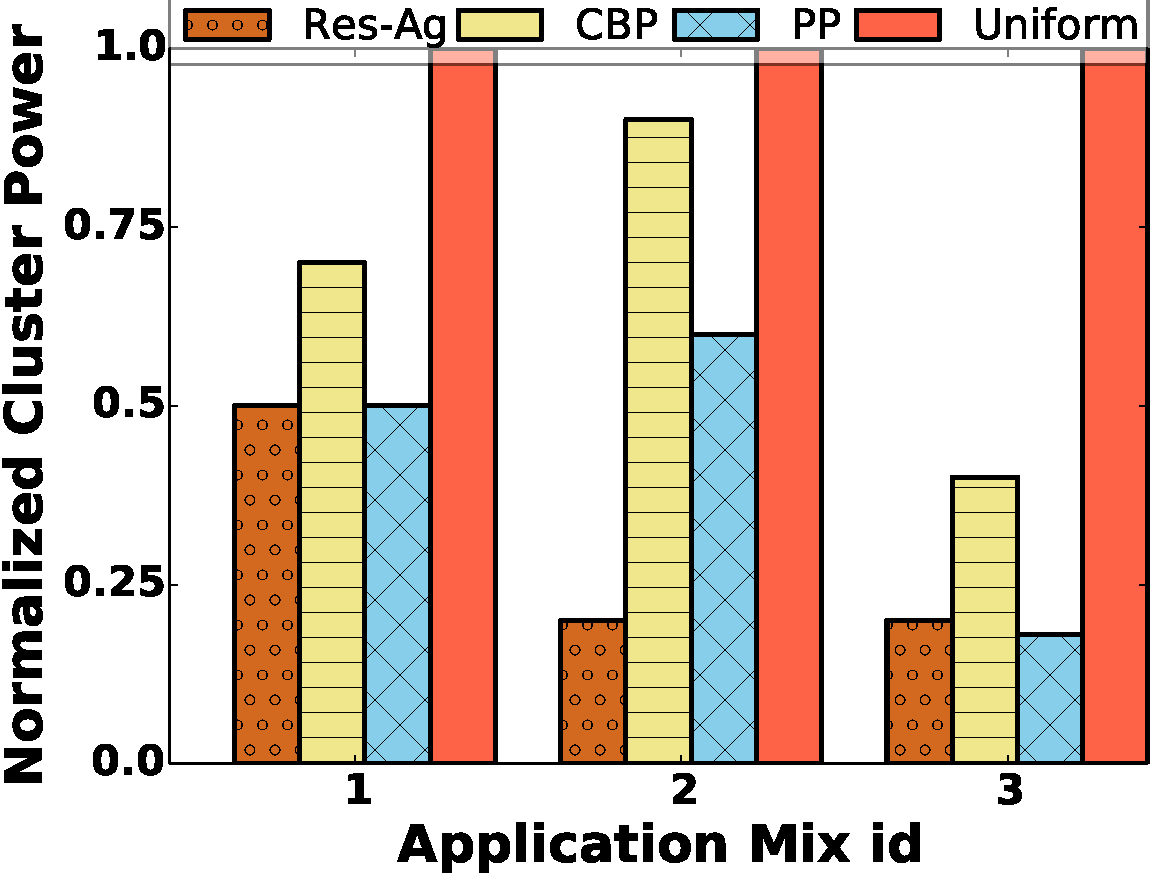
\includegraphics[width=.50\linewidth]{results/power.pdf}
%   \vspace{-2mm}
%   \caption{Normalized power.}
%   \label{fig:power}
% \end{wrapfigure}

% \begin{figure*}
%   \centering
%   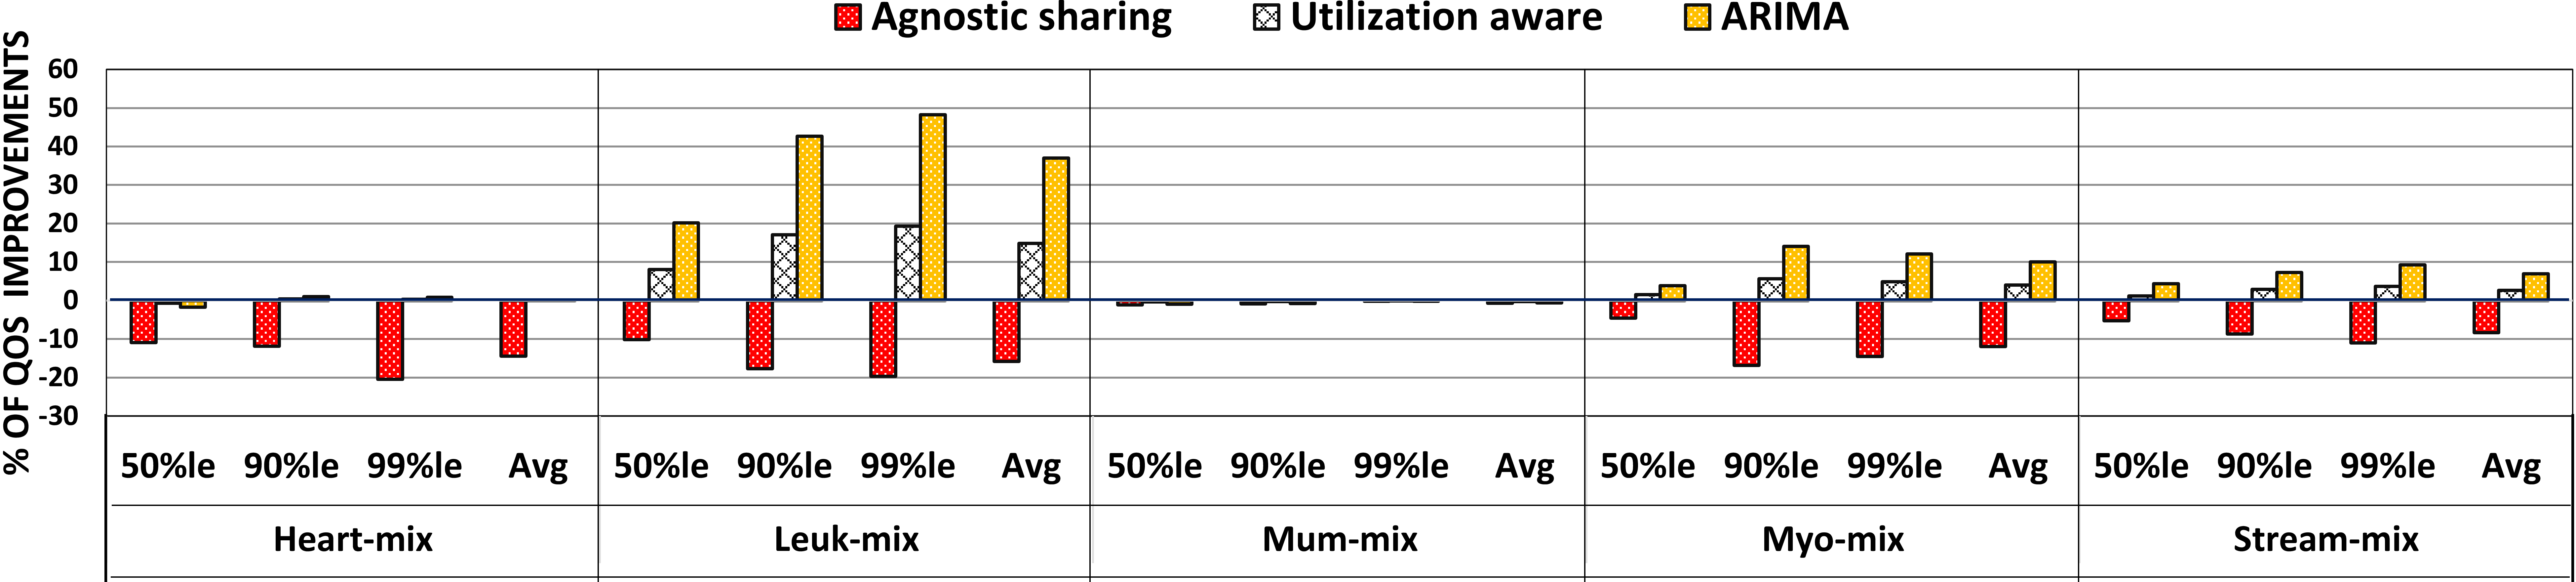
\includegraphics[width=.99\linewidth]{results/scheme.png}
%   \caption{50$^{th}$,90$^{th}$,99$^{th}$ and the average QoS variations plotted for different schedulers for representative mix of workloads compared against default FCFS scheduler.}
%   \label{fig:scheme}
% \end{figure*}

% \vspace{-0.2in}

~\subsection{Accuracy of the Peak Predictor}\label{sec:picking}
In case of PP scheduler, \textit{\textbf{d}} is the frequency at which the utilization aggregator at head-node is querying the worker nodes for GPU utilization that forms our time-series data. We vary the frequency at which we query the GPUs and plot the peak resource usage prediction accuracy in Figure~\ref{fig:accuracy}. As seen, PP improves its accuracy from 40\% to 84\% when the sampling interval for querying utilization is varied from 1000ms to 1 ms, beyond which the accuracy saturates. Hence for the maximum prediction accuracy, we set the utilization aggregator to query the GPU nodes every 1ms. The pyNVML overhead for querying the GPU at 1ms interval was minimal and does not affect the pod's performance. 

\begin{figure}[tbp!]
\begin{subfigure}[b]{.23\textwidth}
  \centering
   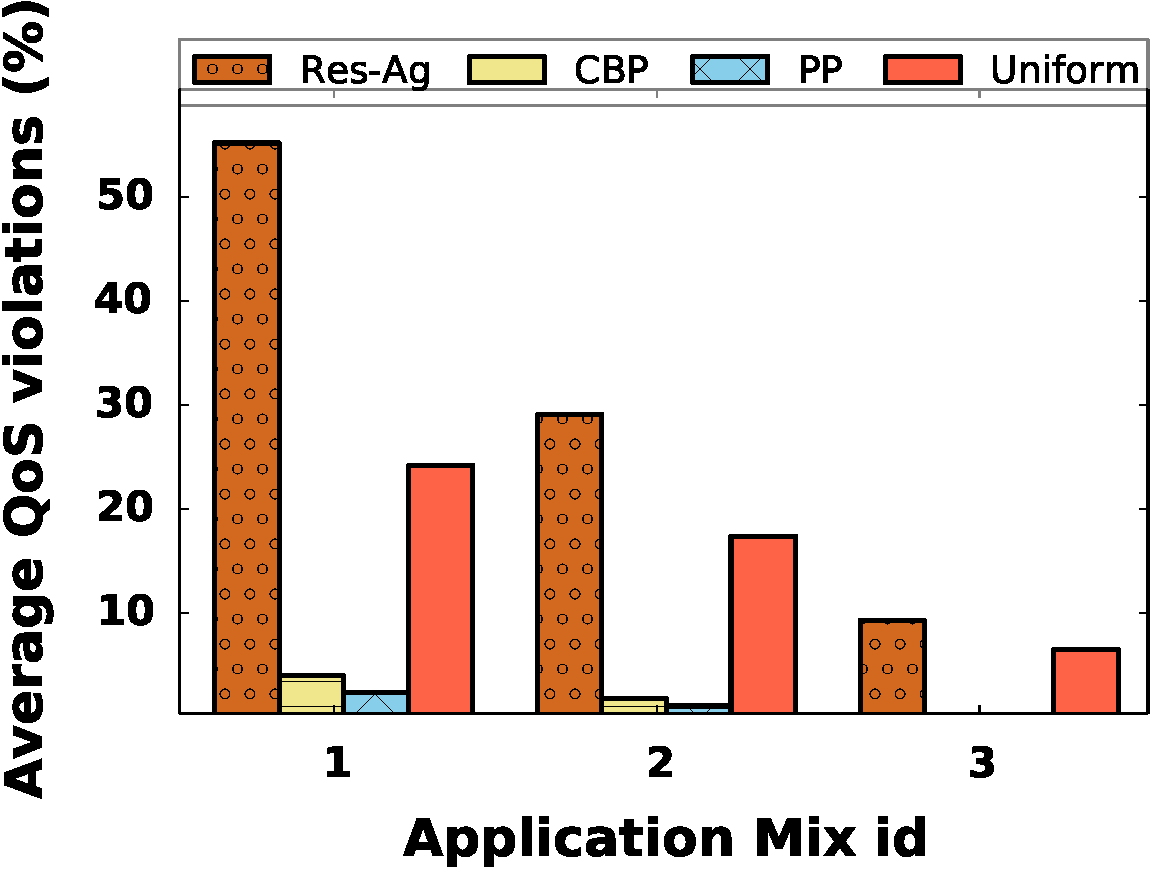
\includegraphics[width=.99\linewidth,height=3.3cm]{figs/qos-1.pdf}
  \caption{Average QoS violations per kilo inferences (queries).}
  \label{fig:qos}
\end{subfigure}
\begin{subfigure}[b]{.23\textwidth}
  \centering
  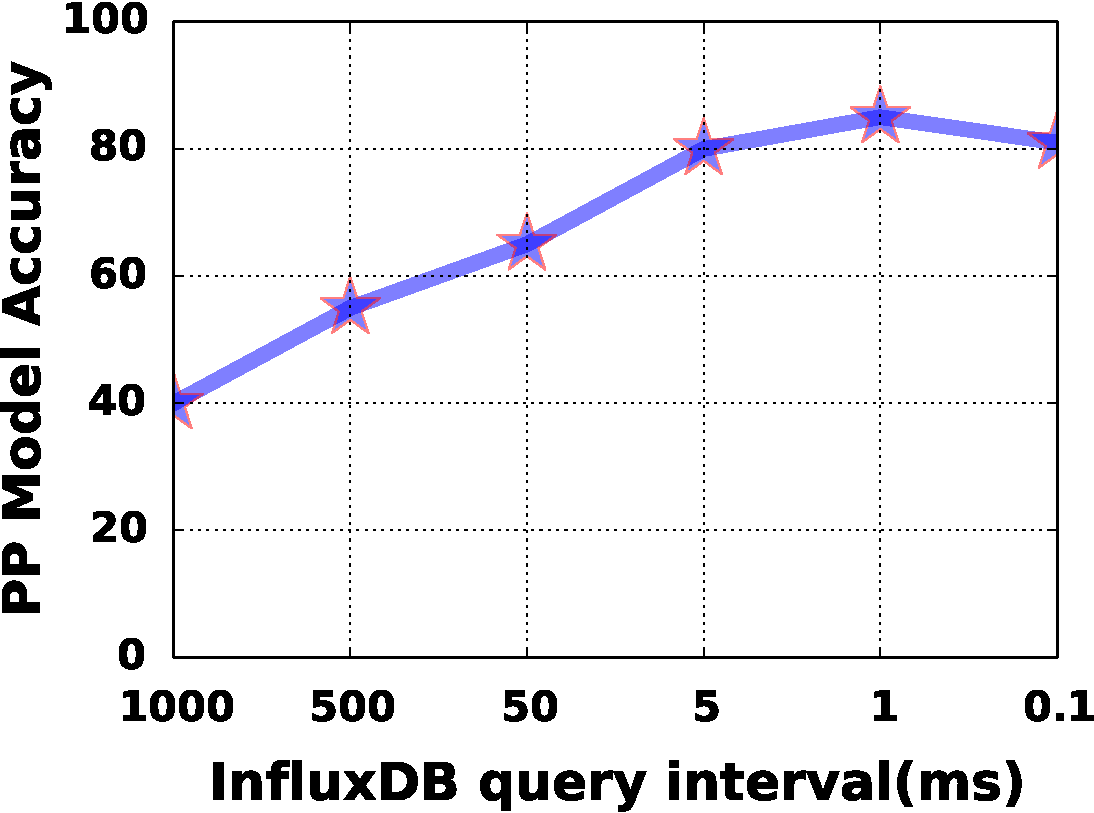
\includegraphics[width=.99\linewidth, height=3.3cm]{figs/accuracy.pdf}
  \caption{Accuracy of PP across varying time intervals in ms.}
  \label{fig:accuracy}
\end{subfigure}
\vspace{-3mm}
\caption{QoS guarantees and Accuracy of PP Scheduler.}
\label{fig:tuning}
\end{figure}

\begin{figure}[tbp!]
\begin{subfigure}[b]{.234\textwidth}
\centering
  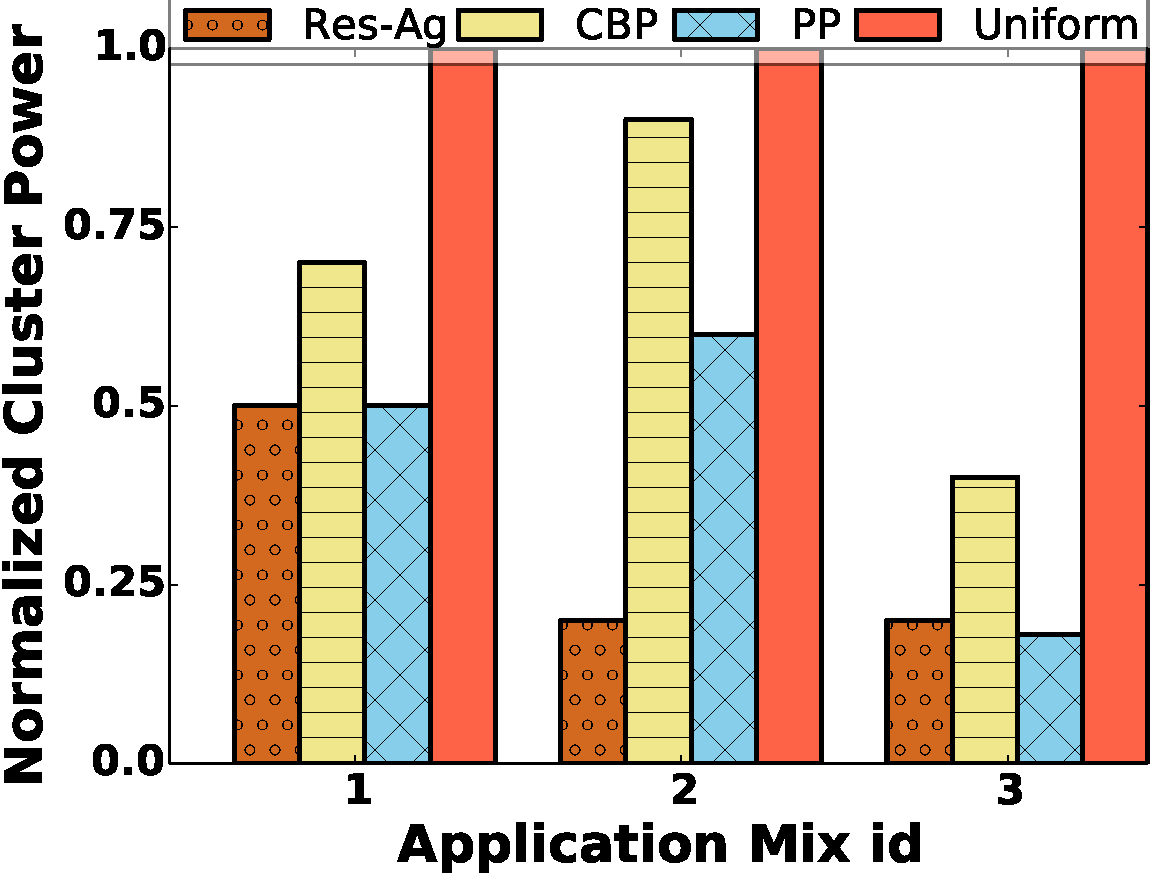
\includegraphics[width=.99\linewidth]{results/power.pdf}
  \caption{Normalized power comparisons across four schedulers.}
  \label{fig:power}
\end{subfigure}
\begin{subfigure}[b]{.234\textwidth}
\centering
  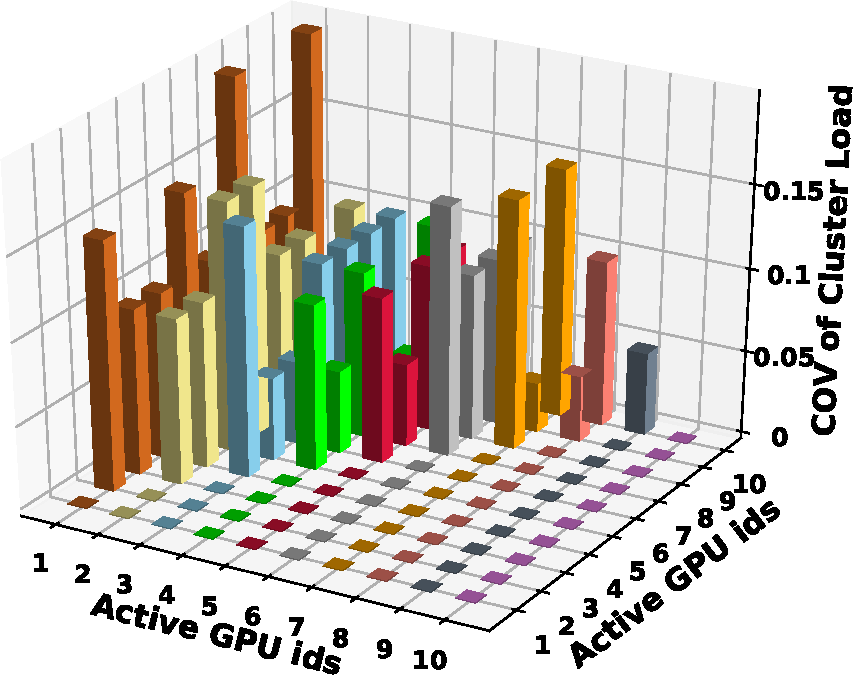
\includegraphics[width=.99\linewidth]{results/active3d.pdf}
  \caption{COV of SM-Load using CBP+PP for App-Mix-1.}
  \label{fig:load}
\end{subfigure}
\vspace{-2mm}
\caption{Cluster-wide Power savings and Load balancing.}
\label{fig:powandload}
\end{figure}



% \vspace{-0.15in}


\subsection{Discussion and Future Work}
\label{sec:overall}

An ideal scheduler would keep all 50/90/99$^{th}$ percentile and max utilization high for all the active GPUs. As a consequence, it yields the best performance per watt spent. This enables the scheduler to analyze different correlation metrics and consolidate the workloads/queries without violating the QoS. However, in reality, this scenario is impractical because of the varying inter-arrival times of GPU jobs submitted in a day. Therefore, the near-optimal solution would be, in every scheduling epoch the scheduler has to ensure performance aware bin-packing while, minimizing the GPU resource fragmentation. This leads to the energy efficient operating point which is achieved by the combination of CBP+PP scheduler.

Our proposed scheduling schemes can potentially be extended to any non-preemptible accelerators such as FPGAs, TPUs to improve the overall utilization while guaranteeing the QoS of the tasks. With the advent of distributed TF-based training~\cite{peng2018optimus,zhang2017slaq,qiao2017litz} on public-cloud GPUs, performance and utilization aware orchestration becomes inevitable to keep the costs low.  

% as input from device-level scheduling the approximate memory bandwidth of an application, by taking the ratio of the total data accesses by its computation kernels to the total time spent on the GPU. Workload balancing uses this information to avoid collocating bandwidth-bound threads. Resulting performance improvements leverage the fact that GPU-resident non-bandwidth/compute-bound threads can hide the memory latencies experienced by bandwidth-bound GPU kernels.


% eak uses a tail bound parameter PB to create the envelope whereas CBP uses a correlation cutoff parameter to identify if two applications are correlated. The baseline settings of all experimental parameters are listed in Table. 2. We evaluate the performance of the proposed methods in comparison with Existing methods based on dynamic consolidation. We run the Existing method with two different sizing functions: (i) Peak Existing sizes all applications based on their peak values and (ii) Mode Existing sizes all applications based on the mode of the distribution. There are three different objectives of consolidation: a)minimize power b) minimize the risk of consolidation (c) balance workload across active servers. We use the number of capacity violations as the metric for risk. To investigate load imbalance, we estimate the average CPU utilization for all active servers during the evaluation period and identify the server with the maximum average CPU utilization. The difference between the CPU utilization of the highest loaded server and the average utilization across all servers is taken as the metric for load imbalance.
% ~\subsubsection{Trading-off accuracy for performance}

%~\subsubsection{Load balancing \& Energy proportionality}
% Recall from the motivation energy plot. Workload Balancing: We next investigate the load balance across the active servers achieved by various methodologies. We observe that Mode Existing and CBP have servers that are always overloaded (average utilization of highest loaded server is 100\%) for AppSuite-1 and AppSuite-2. Such placement is not suitable in practice. Further, for all methodologies other than Peak , there is a large imbalance between the average utilization of the highest loaded server and the average utilization of the cluster. This is a direct consequence of the design of algorithms, where PP favors balancing, and the other algorithms favor creating a skew

%~\subsubsection{Algorithm scalability}

% We also simulate a placement where the initial number of virtual servers on a physical server is increased or decreased. Towards this purpose, we assume that the virtual servers are placed on a different capacity server of the same platform, i.e., with more or fewer processors as required for the simulation. Further, seasonal variations were observed in many workloads and hence, we increase and decrease the training period from the baseline setting. Finally, we vary the tuning parameters of CBP and PP and study their impact.

% ARIMA improves the QoS of service queries by up to 50\% compared to the baseline. This is due to the fact that it can forecast the GPU utilization metrics via the Knots interface. ARIMA does well in cases where the container usage load over time fits into a predictable growth function. This relationship between different load intervals positively correlating with each other could also be observed from the Spearman's correlation of Alibaba traces in Figure~\ref{fig:corr}, which also holds true for GPU.

% ~\subsection{Fragmentation}
% ~\subsubsection{Internal}
% Application managers like Tensorflow, Theano, Torch
% ~\subsubsection{External}
% Fragmentation: We next investigate the ability of CBP and PCP to deal with fragmentation ratio of application capacity to server capacity. We change the original servers in the data center and simulate placement on a larger number of lower capacity servers. In a heterogeneous setting where GPUs like K80 and M40 could be used to reduce external fragmentation issues.









%%------------------------------------------------------------------------------------------------------------------
%% \section{RELATED WORK AND DISCUSSION} 
\section{RELATED WORK} 
\label{sec:related}


GPU resource sharing and over-commitment in datacenters is an emerging research problem. We have done a comprehensive analysis of relevant scheduling frameworks, shown in Table \ref{tbl:related}. Prior works include techniques such as virtualization and runtime support for accelerator management which can be broadly classified into four categories.\\ 
% The community is, however, divided into different design approaches.

\noindent\textbf{Utilization-aware CPU schedulers:}
There are several works that focus on guaranteeing QoS and CPU utilization without sacrificing the SLA of applications. Bubble-up \cite{Marsbubbleup} and Bubble-flux \cite{Yang:bubbleflux} perform safe co-location to avoid interference while improving chip multiprocessor utilization. Prior works such as \cite{Tang:2013:RRS:2451116.2451126} focuses more on resource contention on CPU's in terms of shared memory and shared caches to improve utilization. However, these techniques cannot be directly ported to accelerators. To the best of our knowledge, ours is the first work that considers the GPU's memory usage, bandwidth and SM utilization at the cluster-level to make scheduling and bin-packing decisions.
% However none of the proposed techniques apply to non-preemptive hardware accelerators as the global memory bandwidth of GPU's is different from a CPU. 

\noindent\textbf{Node-level GPU-aware scheduling:}
Recent works ~\cite{gleeson2017heterogeneous,kang2017convgpu} have proposed docker-level container sharing solutions. In this approach, multiple containers can be made to fit in the same GPU as long as the active working set size of all the containers are within the GPU physical memory capacity. 
% which is around 16GB even for NVIDIA's high-end GPUs like Pascal and Volta~\cite{volta}. 
These scheduling techniques over-commit resources for individual containers to ensure crash free execution. This may lead to internal memory fragmentation as we show in Figure~\ref{fig:tf-frag}. We address this by predicting the resource usage and dynamically resizing the containers based on the future resource consumption projections.

\noindent\textbf{GPU-aware runtime systems:}
Researchers have proposed runtime changes to the GPU to enable better scheduling of the GPU tasks either by predicting task behavior or reordering queued tasks.
Ukidave et al.~\cite{ukidave2016mystic} optimized for workloads which under-utilize the device memory and bandwidth. 
Chen et al.~\cite{chen2016baymax} proposed Baymax, a runtime mechanism which does workload batching and kernel reordering to improve the GPU utilization.
% are employed on the host which helps the overall system throughput by mitigating the interference across different kernels when multiple GPU applications run together. 
Other techniques such as interference driven resource management proposed by Phull et al. \cite{Phull:2012:IRM:2287076.2287091}, predicts the interference on a GPU to do safe co-location of GPU tasks. They do not consider memory bandwidth contention nor over-commitment challenges as they assume sequential execution of the GPU tasks. 
% Also they perform static profiling of an application to ensure safe co-locations.
Most of these approaches aim to increase utilization of a individual GPU node and do not scale at the cluster level as they depend on offline training models for node-level run time prediction~\cite{chen2016baymax,ukidave2016mystic}. 
% However, none of these approaches leverage the datacenter wide accelerator heterogeneity which could be achieved only at the resource orchestration layer. Also, both the approaches are at the node-level and have their own merits and demerits. 

\begin{table}[t]
\begin{center}
\resizebox{0.48\textwidth}{!}{%
 \begin{tabular}{||c | c | c | c |c | c | c ||} 
 \hline
 \textbf{Features} & \begin{turn}{90}Baymax \cite{chen2016baymax}\end{turn} & \begin{turn}{90}Prophet \cite{chen2017prophet}\end{turn} & \begin{turn}{90}Quasar \cite{delimitrou2014quasar}\end{turn} & \begin{turn}{90}Mystic \cite{ukidave2016mystic}\end{turn} & \begin{turn}{90}Bubble-Flux \cite{Yang:bubbleflux}\end{turn} & \begin{turn}{90}KubeKnots\end{turn} \\
 \hline
  \textbf{Cluster Level integration } & \xmark & \xmark & \xmark & \xmark & \xmark & {\cmark} \\  
 \hline
 \textbf{Workload consolidation} & \cmark & \cmark & \cmark & \cmark & \cmark & {\cmark} \\  
 \hline
 \textbf{QoS Prediction} & \xmark & \cmark & \cmark & \cmark & \xmark & \xmark \\
 \hline
 \textbf{Utilization Improvement} & \cmark & \cmark & \cmark & \cmark & \cmark & \cmark \\
 \hline
  \textbf{Accelerator power aware} & \xmark & \xmark & \xmark & \xmark & \xmark & \cmark \\
 \hline 
 \textbf{Dynamic Orchestration} & \xmark & \xmark & \xmark & \xmark & \cmark & \cmark \\
 \hline 
 \textbf{Application memory resizing} & \xmark & \xmark & \xmark & \xmark & \xmark & \cmark \\
 \hline 
 \textbf{Application peak prediction} & \xmark & \xmark & \xmark & \xmark & \xmark & \cmark \\
 \hline
\end{tabular}}
\end{center}

  \caption{GPU-based scheduling features comparison.}
  \label{tbl:related}
  \vspace{-3mm}
\end{table}

\noindent\textbf{Hardware support for virtualizing GPUs:}
There has been extensive work on providing hardware support for GPU virtualization ~\cite{Gupta:2011:PCS:2002181.2002184,hong2017gpu} and preemption~\cite{Park:2015:CCP:2694344.2694346,Sajjapongse:2013:PRE:2493123.2462911}. 
% Thread preemption has been proposed to schedule threads for improved utilization selectively. 
Gupta et al.~\cite{Gupta:2011:PCS:2002181.2002184} implemented a task queue in the hypervisor to allow virtualization and preemption of GPU tasks.
Tanasic et al. \cite{Tanasic:2014:EPM:2665671.2665702}  proposed a technique
that improves the performance of high priority processes by enabling preemptive scheduling on GPUs. Aguilera et al. \cite{6742976} proposed a technique to guarantee QoS of high priority tasks by spatially allocating them on more SMs in a GPU. All these techniques require vendors to add extra hardware extensions. Our proposed scheduler does not need any hardware level changes and are readily deployable in Commodity Off-The-Shelf datacenters. We believe ours is the first work at a cluster-level to identify the potential upsides for GPU utilization aware resource orchestration and scheduling (refer Table \ref{tbl:related}).
% and do not work on commodity accelerators. 
% Moreover, provisioning custom accelerators on a public cloud setting is not feasible. 

% However offloading machine learning queries on to the cloud for inference. Since GPUs are non-preemptive, task reordering techniques would fail to work, and hence cannot guarantee the SLO of latency sensitive queries while sticking with the schedule order.


%%------------------------------------------------------------------------------------------------------------------
\section{CONCLUSION} 
\label{sec:conclusion}
In this paper, we observe that the existing resource orchestrators like \textit{Kubernetes} overlook the importance of dynamic orchestration of GPUs. Hence, we identify several challenges in dynamic resource orchestration for GPU-based datacenters.  We explore the possibilities of QoS-aware power proportional scheduling that arise by exposing the GPU APIs to the system orchestrator. Motivated by our observations, we propose \textit{Kube-Knots} by integrating \textit{Knots}, a GPU aware orchestration layer with \textit{Kubernetes} for GPU utilization aware orchestration. We further evaluate three GPU-based scheduling techniques on a ten node GPU-cluster, which leverages \textit{Kube-Knots} for GPU container orchestration.

Our proposed Peak Prediction (PP) scheduler when compared against the \textit{Kubernetes} uniform scheduler, improve the cluster-wide GPU utilization by up to 80\% for both 50$^{th}$ and 90$^{th}$ percentile, through QoS aware workload consolidation which leads to 33\% savings in power consumption across the cluster. Further, we reduced the overall QoS violations of latency sensitive queries by up to 53\% when compared to the resource agnostic scheduler with GPU utilization prediction accuracy as high as at 84\%. We further plan to extend the \textit{Knots} orchestration framework for other accelerators like FPGAs and TPUs.


%However, correlation between co-scheduled GPU applications can lead to significant capacity violations if consolidation methodologies do not take them into account. We design two new placement methodologies which ensures consolidation through CBP and PCP that use an off-peak metric for sizing and another metric to ensure that peaks do not lead to violations. Our experimental evaluation shows that Peak prediction achieves superior power savings, low violations and good load balance across active GPUs in a datacenter.

%-------------------------------------------------------------------------------
\bibliographystyle{plain}
\bibliography{kube-knots}

%%%%%%%%%%%%%%%%%%%%%%%%%%%%%%%%%%%%%%%%%%%%%%%%%%%%%%%%%%%%%%%%%%%%%%%%%%%%%%%%
\end{document}
%%%%%%%%%%%%%%%%%%%%%%%%%%%%%%%%%%%%%%%%%%%%%%%%%%%%%%%%%%%%%%%%%%%%%%%%%%%%%%%%

%%  LocalWords:  endnotes includegraphics fread ptr nobj noindent
%%  LocalWords:  pdflatex acks
